\documentclass[11pt,a4paper]{article}
\usepackage[margin=23mm,headheight=14pt,headsep=8.5mm,footskip=10mm]{geometry}
\usepackage{amsmath,amssymb}
\usepackage{assets/tex/cm-bea}
\usepackage{xeCJK}
\setmainfont{Latin Modern Roman}
\setCJKmainfont{FandolSong-Regular.otf}[Path=assets/fonts/fandol/,BoldFont=FandolSong-Bold.otf,ItalicFont=FandolSong-Regular.otf]
\setCJKsansfont{FandolSong-Regular.otf}[Path=assets/fonts/fandol/,BoldFont=FandolSong-Bold.otf]
\xeCJKsetup{PunctStyle=quanjiao,CheckSingle=true}
\usepackage{setspace}\setstretch{1.12}
\setlength{\parindent}{2em}\setlength{\parskip}{3pt}
\usepackage{titlesec}
\titleformat{\section}{\centering\normalfont\large\bfseries}{}{0pt}{}
\titleformat{\subsection}{\normalfont\normalsize\bfseries}{}{0pt}{}
\titlespacing*{\section}{0pt}{1.5\baselineskip}{0.8\baselineskip}
\titlespacing*{\subsection}{0pt}{1.1\baselineskip}{0.5\baselineskip}
\usepackage{needspace,enumitem,longtable,booktabs,array,calc,graphicx}
\providecommand{\tightlist}{\setlength{\itemsep}{3pt}\setlength{\parskip}{0pt}}
\usepackage{fancyhdr}\pagestyle{fancy}\fancyhf{}
\fancyhead[L]{\small 曲线积分与曲面积分}\fancyhead[R]{\small\hyperlink{lecture-toc}{目录}}
\fancyfoot[C]{\thepage}\renewcommand{\headrulewidth}{0.4pt}
\usepackage[hidelinks,unicode,linktoc=all]{hyperref}\usepackage{bookmark}
\hypersetup{pdfauthor={Vincent Arqain},pdftitle={曲线积分与曲面积分}}
\renewcommand{\contentsname}{目录}\setcounter{tocdepth}{2}\setcounter{secnumdepth}{0}
\widowpenalty=10000\clubpenalty=10000\displaywidowpenalty=10000
\predisplaypenalty=10000\interdisplaylinepenalty=1000
\raggedbottom\emergencystretch=2em
\setlength{\LTpre}{6pt}\setlength{\LTpost}{6pt}
\newcommand{\fig}[2]{\begin{center}\includegraphics[width=0.76\linewidth,height=0.34\textheight,keepaspectratio]{print/curve-surface-figures/#1.pdf}\par\small #2\end{center}}

\input{ot1cmss.fd}
\DeclareFontShape{OT1}{cmss}{b}{n}{<->ssub*cmss/bx/n}{}
\DeclareFontShape{OT1}{cmss}{b}{it}{<->ssub*cmss/bx/n}{}
\DeclareFontShape{OT1}{cmss}{bx}{it}{<->ssub*cmss/bx/n}{}
\usepackage{bm,xcolor,tikz,etoolbox,xstring}
\usetikzlibrary{arrows.meta,decorations.markings}
\definecolor{navy}{RGB}{31,30,29}\definecolor{ink}{RGB}{31,30,29}
\newcommand{\dd}{\mathop{}\!\mathrm d}
\newcommand{\vct}[1]{\bm{#1}}\newcommand{\rr}{\vct r}\newcommand{\FF}{\vct F}\newcommand{\nn}{\vct n}\newcommand{\ttau}{\vct\tau}
\DeclareMathOperator{\grad}{grad}\DeclareMathOperator{\diver}{div}\DeclareMathOperator{\rot}{rot}\DeclareMathOperator{\curl}{curl}\DeclareMathOperator{\arcosh}{arcosh}
\makeatletter
\newcommand{\oiint}{\mathop{\mathpalette\closed@double\relax}\nolimits}
\newcommand{\closed@double}[2]{\ooalign{$\m@th#1\iint$\cr\hidewidth\raisebox{0.02ex}{$\m@th#1\circ$}\hidewidth\cr}}
\makeatother
\newcommand{\src}[1]{\par{\footnotesize 出处：原书 #1。纸书页码；原 PDF 页码加 11。}\par}
\newcommand{\entry}[3]{\IfBeginWith{#1}{例}{\def\entrytitle{*#1}}{\def\entrytitle{#1}}\Needspace{6\baselineskip}\subsection*{\entrytitle\quad #2}\phantomsection\addcontentsline{toc}{subsection}{\entrytitle\quad #2}\src{#3}}
\newcommand{\ednote}[1]{\par{\small\textbf{编校注}\quad #1}\par}
\newcommand{\sol}{\par\textbf{原解}\quad}\newcommand{\prooftext}{\par\textbf{原证明}\quad}
\setlist[itemize]{leftmargin=1.4em,label={},itemsep=3pt,topsep=3pt,parsep=1pt}
\setlist[enumerate]{leftmargin=2.5em,label=(\roman*),itemsep=3pt,topsep=3pt}
\setcounter{secnumdepth}{1}\renewcommand{\thesection}{§A.\arabic{section}}
\titleformat{\section}{\centering\normalfont\large\bfseries}{\thesection}{0.6em}{}
\makeatletter
\renewcommand*\l@section{\@dottedtocline{1}{0em}{3.8em}}
\renewcommand*\l@subsection{\@dottedtocline{2}{1.5em}{0em}}
\makeatother
\pretocmd{\section}{\Needspace{7\baselineskip}}{}{}
\hypersetup{pdftitle={曲线积分与曲面积分讲义：58 道带星号原例题阅读附录}}
\begin{document}
\begin{center}{\LARGE\bfseries 曲线积分与曲面积分讲义\par}\vspace{7pt}
{\large 独立阅读附录：58 道带星号原例题\par}\end{center}
本册根据用户上传的《多元积分计算》PDF 及其对应源码编排。58 道例题全部保留，题目前加“*”；原题号、计算过程、原证明、图形和编校注保持原样。原资料中的定义、定理和反常积分内容同时保留，以便独立阅读。本册不纳入讲义正文 §1—§11，也不计入正文的 16 道科大精选例题。

原资料出处：佘志坤主编，全国大学生数学竞赛命题组编，《全国大学生数学竞赛解析教程（数学专业类）（上册）——数学分析》，科学出版社，2024。纸书页码见各条出处。

原文件中“原解存疑”等编校说明继续保留，尤其 *例 5.2.12；保留原解不表示这些条目已被重新确认正确。全册中文采用 Fandol 宋体，数学公式统一为 CM bea。
\hypertarget{lecture-toc}{}\begingroup\small\setlength{\parskip}{0pt}\tableofcontents\endgroup\clearpage
\section{曲线积分：基本概念及性质}
\entry{定义 5.2.1}{第一型曲线积分}{p.258}
设 $L$ 为 $\mathbb R^3$ 中可求长曲线，端点为 $A,B$。依次取分点
\[
A=A_0,A_1,\ldots,A_n=B,
\]
构成分割 $T$；弧段 $L_i=A_{i-1}A_i$ 的弧长记为 $\Delta s_i$，分割细度为 $\lambda=\max_i\Delta s_i$。在 $L_i$ 上任取 $P_i=(\xi_i,\eta_i,\zeta_i)$，令
\[
S(f,T)=\sum_{i=1}^n f(P_i)\Delta s_i.
\]
若存在 $I$，使任意 $\varepsilon>0$，存在 $\delta>0$，只要 $\lambda<\delta$，不论介点如何选择，均有 $|S(f,T)-I|<\varepsilon$，则称 $f$ 在 $L$ 上可积，记为
\[
I=\int_L f(x,y,z)\dd s=\int_L f\dd s.
\]
\begin{center}\begin{minipage}{\linewidth}\centering
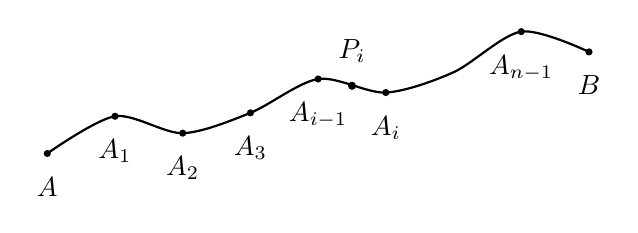
\begin{tikzpicture}[scale=.86]
\draw[thick] plot[smooth] coordinates {(0,0)(1,.55)(2,.3)(3,.6)(4,1.1)(5,.9)(6,1.2)(7,1.8)(8,1.5)};
\foreach \x/\y/\lab in {0/0/A,1/.55/A_1,2/.3/A_2,3/.6/A_3,4/1.1/A_{i-1},5/.9/A_i,7/1.8/A_{n-1},8/1.5/B}{\fill (\x,\y) circle(1.5pt) node[below=5pt] {$\lab$};}
\fill (4.5,1) circle(1.7pt) node[above=5pt] {$P_i$};
\end{tikzpicture}
\par{\small 图 5.2.1\quad 曲线分割示意（重绘）}
\end{minipage}\end{center}

\entry{定义 5.2.2}{第二型曲线积分}{p.259}
设 $\FF=(P,Q,R)$ 为空间区域 $D$ 中的向量场，$L\subset D$ 为从 $A$ 到 $B$ 的可求长有向曲线。顺序取分点 $\rr_0=A,\ldots,\rr_n=B$，记
\[
\Delta\rr_i=\rr_i-\rr_{i-1},\qquad \|T\|=\max_i|\Delta\rr_i|.
\]
在各弧段上任取 $\vct\xi_i$，若极限
\[
\lim_{\|T\|\to0}\sum_{i=1}^n\FF(\vct\xi_i)\cdot\Delta\rr_i
\]
为定数，则记为 $\int_L\FF\cdot\dd\rr$。闭曲线 $L$ 上的积分称为环量，记为 $\oint_L\FF\cdot\dd\rr$。因 $\rr=(x,y,z)$、$\dd\rr=(\dd x,\dd y,\dd z)$，也记为
\[
\int_L\FF\cdot\dd\rr=\int_L P\dd x+Q\dd y+R\dd z.
\]

\entry{定理 5.2.1}{第一型曲线积分的参数计算}{p.259}
设 $L\subset\mathbb R^3$ 为光滑曲线，其参数为
$\vct\varphi(t)=(x(t),y(t),z(t))$，$\alpha\le t\le\beta$，且 $f$ 在 $L$ 上连续，则
\[
\int_L f\dd s=\int_\alpha^\beta(f\circ\vct\varphi)(t)|\vct\varphi'(t)|\dd t.
\]
\textbf{注 5.2.1}\quad 此公式将第一型曲线积分化为区间上的 Riemann 积分。

\entry{定理 5.2.2}{第二型曲线积分的参数计算}{pp.259—260}
设 $D\subset\mathbb R^3$ 为区域，$\FF:D\to\mathbb R^3$ 连续，$L\subset D$ 为有向光滑曲线，参数 $\rr=\rr(t)$，$\alpha\le t\le\beta$，参数增加方向与 $L$ 一致，则
\[
\int_L\FF\cdot\dd\rr=\int_\alpha^\beta(\FF\circ\rr)(t)\cdot\rr'(t)\dd t.
\]
当 $\FF=(P,Q,R)$ 时，右端为
\[
\int_\alpha^\beta\bigl[P(\rr(t))x'(t)+Q(\rr(t))y'(t)+R(\rr(t))z'(t)\bigr]\dd t.
\]
\textbf{注 5.2.2}\quad 此公式将第二型曲线积分化为区间上的 Riemann 积分。

\entry{性质}{第二型曲线积分的基本性质}{p.260}
\textbf{（1）线性。} 若 $\FF=c_1\FF_1+c_2\FF_2$，则
\[
\int_L\FF\cdot\dd\rr=c_1\int_L\FF_1\cdot\dd\rr+c_2\int_L\FF_2\cdot\dd\rr.
\]
特别地，对 $\FF_1=P\vct i$、$\FF_2=Q\vct j$、$\FF_3=R\vct k$，有
\[
\int_L\FF\cdot\dd\rr=\int_L P\dd x+Q\dd y+R\dd z
=\int_L P\dd x+\int_L Q\dd y+\int_L R\dd z.
\]
\textbf{（2）路径可加性。} 若 $L_{AC}$ 由 $L_{AB}$ 与 $L_{BC}$ 连接而成，则
\[
\int_{L_{AC}}\FF\cdot\dd\rr=\int_{L_{AB}}\FF\cdot\dd\rr+\int_{L_{BC}}\FF\cdot\dd\rr.
\]
因此，逐段光滑曲线可以分段积分。

\textbf{（3）方向性。}
\[
\int_{L_{AB}}\FF\cdot\dd\rr=-\int_{L_{BA}}\FF\cdot\dd\rr.
\]

\entry{定理 5.2.3}{Green 公式}{p.260}
设 $D$ 为有限条逐段光滑封闭曲线 $L$ 围成的平面闭区域，$\FF=(P(x,y),Q(x,y))$ 为 $D$ 上光滑场，则
\[
\oint_L P\dd x+Q\dd y=\iint_D\left(\frac{\partial Q}{\partial x}-\frac{\partial P}{\partial y}\right)\dd x\dd y,
\]
其中 $L=\partial D$ 取行进时 $D$ 在左侧的方向。

\entry{定义 5.2.3}{有势场与势函数}{p.260}
设 $\FF=(P,Q,R)$ 定义于 $V\subset\mathbb R^3$。若存在数量场 $\varphi$，使
\[
\grad\varphi(\vct p)=\FF(\vct p),\qquad\forall\vct p\in V,
\]
则称 $\FF$ 有势，$\varphi$ 为势函数，即 $\varphi_x=P$、$\varphi_y=Q$、$\varphi_z=R$。

\entry{定义 5.2.4}{保守场}{p.260}
若 $\FF$ 对 $V$ 内任意有向闭路 $L$ 均有 $\oint_L\FF\cdot\dd\rr=0$，则称 $\FF$ 为保守场。

\entry{定理 5.2.4}{保守与有势}{p.261}
向量场保守的充要条件为有势。

\entry{定理 5.2.5}{无旋与有势的判据}{p.261}
在曲面单连通的区域 $V$ 上，光滑向量场 $\FF$ 是有势场的充要条件是它是无旋场，即在 $V$ 中每点 $\rot(\FF)$ 是零向量。
\ednote{原书作“曲面单连通”；此处有势判据通常要求路径（线）单连通，使用时应核对区域假设。}

\clearpage
\section{曲线积分：例题及原解}
\entry{例 5.2.1}{圆周上的第一型积分}{p.261}
求 $I=\int_L\sqrt{x^2+y^2}\dd s$，其中 $L:x^2+y^2=ax$，$a>0$。
\sol 取参数
\[
x=\frac a2+\frac a2\cos t,\quad y=\frac a2\sin t,\quad 0\le t\le2\pi.
\]
则 $\rr'(t)=(-\frac a2\sin t,\frac a2\cos t)$，$\dd s=\frac a2\dd t$。于是
\[
I=\frac{a^2}{2}\int_0^{2\pi}\left|\cos\frac t2\right|\dd t
=a^2\int_0^\pi|\cos t|\dd t=2a^2.
\]
\ednote{原书首个代入式根号内疑多一因子 $a$；此处按所列参数式与后续等式整理，仅保留原解后续正确计算链。}

\entry{例 5.2.2}{第一象限椭圆弧}{p.261}
设 $L$ 为 $x^2/a^2+y^2/b^2=1$（$a,b>0$）在第一象限的弧，求 $\int_Lxy\dd s$。
\sol 令 $x=a\cos\theta$，$y=b\sin\theta$，$0\le\theta\le\pi/2$，则
\begin{align*}
I&=ab\int_0^{\pi/2}\cos\theta\sin\theta\sqrt{a^2\sin^2\theta+b^2\cos^2\theta}\dd\theta\\
&=\frac{ab}{2}\int_0^{\pi/2}\sqrt{b^2+(a^2-b^2)\sin^2\theta}\dd(\sin^2\theta)\\
&=\frac{ab}{2}\int_0^1\sqrt{b^2+(a^2-b^2)t}\dd t
=\frac{ab(a^2+ab+b^2)}{3(a+b)}.
\end{align*}

\entry{例 5.2.3}{三角形边界上的弧长积分}{pp.261—262}
求 $\int_Lx\dd s$，其中 $L$ 为 $O(0,0)$、$A(1,0)$、$B(0,1)$ 所成三角形的边界。
\sol 将曲线分段，均取 $0\le t\le1$：
\[
\begin{array}{c|ccc}
 &x&y&\dd s\\\hline
OA&t&0&\dd t\\
AB&1-t&t&\sqrt2\dd t\\
BO&0&1-t&\dd t
\end{array}
\]
因此
\begin{align*}
I&=\int_{OA}x\dd s+\int_{AB}x\dd s+\int_{BO}x\dd s\\
&=\int_0^1t\dd t+\int_0^1(1-t)\sqrt2\dd t+\int_0^10\dd t
=\frac{1+\sqrt2}{2}.
\end{align*}
\begin{center}\begin{minipage}{\linewidth}\centering
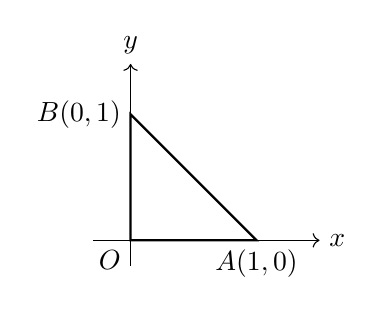
\begin{tikzpicture}[scale=1.6]
\draw[->](-.3,0)--(1.5,0)node[right]{$x$};\draw[->](0,-.2)--(0,1.4)node[above]{$y$};
\draw[thick](0,0)--(1,0)--(0,1)--cycle;
\node[below left]at(0,0){$O$};\node[below]at(1,0){$A(1,0)$};\node[left]at(0,1){$B(0,1)$};
\end{tikzpicture}\par{\small 图 5.2.2\quad 三角形边界（重绘）}
\end{minipage}\end{center}

\entry{例 5.2.4}{球面与平面交圆的对称性}{p.262}
求 $I=\int_Lxy\dd s$，其中 $L$ 为球面 $x^2+y^2+z^2=a^2$ 与平面 $x+y+z=0$ 的交圆。
\sol 由对称性，$\int_Lxy\dd s=\int_Lyz\dd s=\int_Lzx\dd s$。因此
\begin{align*}
I&=\frac13\int_L(xy+yz+zx)\dd s\\
&=\frac16\int_L\bigl[(x+y+z)^2-(x^2+y^2+z^2)\bigr]\dd s\\
&=-\frac16\int_La^2\dd s=-\frac16a^2\cdot2\pi a=-\frac{\pi a^3}{3}.
\end{align*}

\entry{例 5.2.5}{锥面与柱面交线上的积分}{pp.262—263}
求 $I=\int_Lz\dd s$，其中 $L$ 为 $x^2+y^2=z^2$ 和 $y^2=ax$（$a>0$）的交线从 $(0,0,0)$ 到 $(a,a,a\sqrt2)$ 的弧。
\sol 取 $y=t$，则
\[
\rr(t)=\left(\frac{t^2}{a},t,\frac{t\sqrt{t^2+a^2}}{a}\right),\quad 0\le t\le a,
\qquad |\rr'(t)|=\frac1a\sqrt{\frac{8t^4+9a^2t^2+2a^4}{t^2+a^2}}.
\]
于是
\begin{align*}
I&=\int_0^a\frac{t\sqrt{t^2+a^2}}a\cdot\frac1a\sqrt{\frac{8t^4+9a^2t^2+2a^4}{t^2+a^2}}\dd t\\
&=\frac1{a^2}\int_0^at\sqrt{8t^4+9a^2t^2+2a^4}\dd t\\
&=\frac1{2a^2}\int_0^{a^2}\sqrt{8t^2+9a^2t+2a^4}\dd t\\
&=\frac{\sqrt2}{a^2}\int_0^{a^2}\sqrt{\left(t+\frac{9a^2}{16}\right)^2-\left(\frac{\sqrt{17}a^2}{16}\right)^2}\dd t.
\end{align*}
令 $u=t+9a^2/16$，$b=\sqrt{17}a^2/16$，则
\begin{align*}
I&=\frac{\sqrt2}{a^2}\int_{9a^2/16}^{25a^2/16}\sqrt{u^2-b^2}\dd u\\
&=\frac{17\sqrt2a^2}{256}\int_{9/\sqrt{17}}^{25/\sqrt{17}}\sqrt{t^2-1}\dd t\\
&=\frac{\sqrt2a^2}{512}\left[100\sqrt{38}-72-17\arcosh\frac{25}{\sqrt{17}}+17\arcosh\frac9{\sqrt{17}}\right].
\end{align*}

\entry{例 5.2.6}{三角形正向周界的第二型积分}{p.263}
求 $I=\oint_Lxy\dd x+x^2\dd y$，其中 $L$ 为 $O(0,0)$、$A(1,2)$、$B(0,2)$ 所成三角形的正向周界。
\sol 分为 $L_1=OA$、$L_2=AB$、$L_3=BO$，有
\begin{align*}
\int_{L_1}xy\dd x+x^2\dd y&=\int_0^1(x\cdot2x+2x^2)\dd x=4\int_0^1x^2\dd x=\frac43,\\
\int_{L_2}xy\dd x+x^2\dd y&=-2\int_0^1(1-x)\dd x=-1,\\
\int_{L_3}xy\dd x+x^2\dd y&=0.
\end{align*}
故 $I=4/3-1=1/3$。
\begin{center}\begin{minipage}{\linewidth}\centering
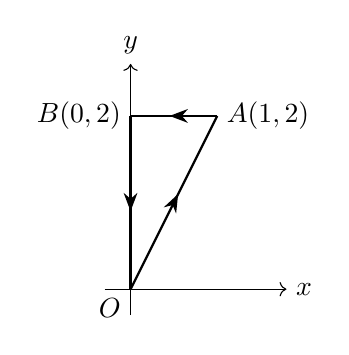
\begin{tikzpicture}[scale=1.1,midarrow/.style={postaction={decorate},decoration={markings,mark=at position .55 with {\arrow{Stealth}}}}]
\draw[->](-.3,0)--(1.8,0)node[right]{$x$};\draw[->](0,-.3)--(0,2.6)node[above]{$y$};
\draw[thick,midarrow](0,0)--(1,2);\draw[thick,midarrow](1,2)--(0,2);\draw[thick,midarrow](0,2)--(0,0);
\node[below left]at(0,0){$O$};\node[right]at(1,2){$A(1,2)$};\node[left]at(0,2){$B(0,2)$};
\end{tikzpicture}\par{\small 图 5.2.3\quad 有向三角形（重绘）}
\end{minipage}\end{center}

\entry{例 5.2.7}{球面与过轴平面的有向交圆}{pp.263—264}
求
\[
I=\oint_L(y-z)\dd x+(z-x)\dd y+(x-y)\dd z,
\]
其中 $L$ 为球面 $x^2+y^2+z^2=R^2$ 与平面 $y=x\tan\alpha$ 的交圆，从 $x$ 轴正向看去为顺时针，$0<\alpha<\pi/2$。
\sol 球面的参数为
\[
x=R\sin\theta\cos\varphi,\quad y=R\sin\theta\sin\varphi,\quad z=R\cos\theta,
\quad 0\le\theta\le\pi,\quad0\le\varphi\le2\pi.
\]
因 $L$ 又在平面上，故 $\tan\varphi=\tan\alpha$，即 $\varphi=\alpha$ 或 $\pi+\alpha$。两半圆为
\[
\begin{aligned}
L_1:\ &x=R\sin\theta\cos\alpha,\quad y=R\sin\theta\sin\alpha,\quad z=R\cos\theta,\\
L_2:\ &x=-R\sin\theta\cos\alpha,\quad y=-R\sin\theta\sin\alpha,\quad z=-R\cos\theta,
\end{aligned}\qquad 0\le\theta\le\pi.
\]
于是可以统一写为 $x=R\sin\theta\cos\alpha$、$y=R\sin\theta\sin\alpha$、$z=R\cos\theta$，$0\le\theta\le2\pi$。代入得
\begin{align*}
I=\int_0^{2\pi}\bigl[&(R\sin\theta\sin\alpha-R\cos\theta)(R\cos\theta\cos\alpha)\\
&+(R\cos\theta-R\sin\theta\cos\alpha)(R\cos\theta\sin\alpha)\\
&+(R\sin\theta\cos\alpha-R\sin\theta\sin\alpha)(-R\sin\theta)\bigr]\dd\theta\\
=R^2\int_0^{2\pi}&(\sin\alpha-\cos\alpha)\dd\theta=2\pi(\sin\alpha-\cos\alpha)R^2.
\end{align*}
\begin{center}\begin{minipage}{\linewidth}\centering
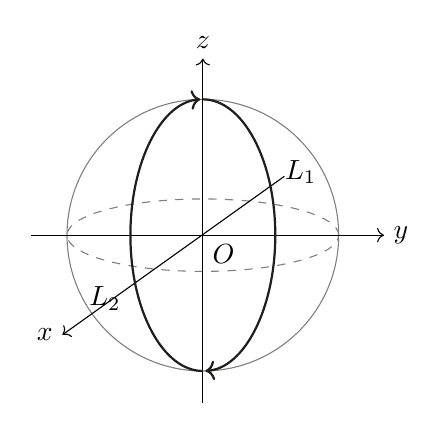
\begin{tikzpicture}[scale=1.15]
\draw[gray] (0,0)circle(1.5);\draw[gray,dashed](0,0)ellipse(1.5 and .4);
\draw[->](-1.9,0)--(2,0)node[right]{$y$};\draw[->](.9,.65)--(-1.55,-1.1)node[left]{$x$};\draw[->](0,-1.85)--(0,1.95)node[above]{$z$};
\draw[thick,navy,->](0,1.5) arc[start angle=90,end angle=-88,x radius=.8,y radius=1.5];
\draw[thick,navy,->](0,-1.5) arc[start angle=270,end angle=92,x radius=.8,y radius=1.5];
\node[right]at(.8,.7){$L_1$};\node[left]at(-.8,-.7){$L_2$};\node[below right]at(0,0){$O$};
\end{tikzpicture}\par{\small 图 5.2.4\quad 球面及有向交圆的投影示意（重绘，非按比例）}
\end{minipage}\end{center}

\entry{例 5.2.8}{路径无关确定函数}{pp.264—265}
设 $f$ 有连续导数，$f(0)=0$，且
\[
\int_C(e^x+f(x))y\dd x+f(x)\dd y
\]
与路径无关，求从 $(0,0)$ 到 $(1,1)$ 的积分。
\sol 路径无关的条件为 $f'(x)-(e^x+f(x))=0$。解得
$f(x)=xe^x+Ce^x$。由 $f(0)=0$，得 $C=0$，故 $f(x)=xe^x$。
将积分路径改为 $(0,0)\to(1,0)\to(1,1)$，则积分等于
\[
0+\int_0^1 f(1)\dd y=f(1)=e.
\]

\entry{例 5.2.9}{Green 公式与非负积分}{p.265}
设 $L:(x-1)^2+(y-1)^2=1$ 取逆时针方向，$f$ 为正值可微函数，且
\[
\oint_L\frac{y}{f(x)}\dd x+xf(y)\dd y=2\pi,
\]
求 $f$。
\sol 设 $D$ 为圆内区域。由 Green 公式，
\[
I=\iint_D\left[f(y)+\frac1{f(x)}\right]\dd x\dd y.
\]
由于 $D$ 关于 $x,y$ 对称，亦有 $I=\iint_D[f(x)+1/f(y)]\dd x\dd y$。故
\[
I=\frac12\iint_D\left[f(x)+f(y)+\frac1{f(x)}+\frac1{f(y)}\right]\dd x\dd y.
\]
又 $I=2\pi=2\iint_D\dd x\dd y$，推出
\[
\iint_D\left[\left(\sqrt{f(x)}-\frac1{\sqrt{f(x)}}\right)^2
+\left(\sqrt{f(y)}-\frac1{\sqrt{f(y)}}\right)^2\right]\dd x\dd y=0.
\]
因此 $\sqrt{f(x)}-1/\sqrt{f(x)}=0$，即 $f(x)=1$。
\ednote{原书结论未写取值域；上述推导约束的是圆域投影内的 $f$ 值，不能据此擅自断言全实轴上均成立。}

\entry{例 5.2.10}{参数曲线围成区域的面积}{pp.265—266}
设 $a,b,c>0$，求曲线
\[
L:\left(\frac xa\right)^{2n+1}+\left(\frac yb\right)^{2n+1}
=c\left(\frac xa\right)^n\left(\frac yb\right)^n
\]
围成区域 $D$ 的面积 $\sigma(D)$。
\sol 令 $t=ay/(bx)$，得到参数式
\[
x(t)=\frac{ac\,t^n}{t^{2n+1}+1},\quad y(t)=\frac{bc\,t^{n+1}}{t^{2n+1}+1},\quad t\in[0,+\infty).
\]
由 Green 公式，
\begin{align*}
\sigma(D)&=\frac12\oint_L(-y\dd x+x\dd y)
=\frac12\int_0^\infty[x(t)y'(t)-x'(t)y(t)]\dd t\\
&=\frac12\int_0^\infty\frac{abc^2t^{2n}}{(t^{2n+1}+1)^2}\dd t
=\frac{abc^2}{2(2n+1)}.
\end{align*}

\entry{例 5.2.11}{两椭圆公共区域的面积}{pp.266—267}
求平面椭圆 $L_1:x^2/a^2+y^2/b^2=1$ 与 $L_2:x^2/b^2+y^2/a^2=1$（$a>b$）内部公共区域的面积。
\sol 由对称性，只算第一象限的公共区域 $D$。原书称 $L_1$ 与 $x$ 轴交于 $B$，$L_2$ 与 $y$ 轴交于 $A$，两椭圆交于 $P$，并给出
\[
A=(0,b),\quad B=(b,0),\quad P=\left(\frac{ab}{\sqrt{a^2+b^2}},\frac{ab}{\sqrt{a^2+b^2}}\right).
\]
原书记边界为 $OB$、$L_1$ 上弧 $BP$、$L_2$ 上弧 $PA$、$AO$；随后取参数
\[
\begin{aligned}
BP:&\quad x=b\cos\varphi,\quad y=a\sin\varphi,\quad 0\le\varphi\le\arctan(b/a),\\
PA:&\quad x=a\cos\varphi,\quad y=b\sin\varphi,\quad \arctan(a/b)\le\varphi\le\pi/2.
\end{aligned}
\]
\ednote{原书此处弧段的 $L_1/L_2$ 文字标号与随后参数疑互换；上列参数照录。轴交点应结合所给坐标与参数理解，图中按几何实际绘制。}
在 $OB$、$AO$ 上有 $-y\dd x+x\dd y=0$，因而
\[
\sigma(D)=\frac12\oint_{\partial D}(-y\dd x+x\dd y)
=\frac12\int_{BP}(-y\dd x+x\dd y)+\frac12\int_{PA}(-y\dd x+x\dd y).
\]
其中
\begin{align*}
\int_{BP}(-y\dd x+x\dd y)&=\int_0^{\arctan(b/a)}(ab\cos^2\varphi+ab\sin^2\varphi)\dd\varphi\\
&=ab\arctan(b/a),\\
\int_{PA}(-y\dd x+x\dd y)&=\int_{\arctan(a/b)}^{\pi/2}ab\dd\varphi\\
&=ab\bigl(\pi/2-\arctan(a/b)\bigr)=ab\arctan(b/a).
\end{align*}
所以所求总面积为 $4ab\arctan(b/a)$。
\begin{center}\begin{minipage}{\linewidth}\centering
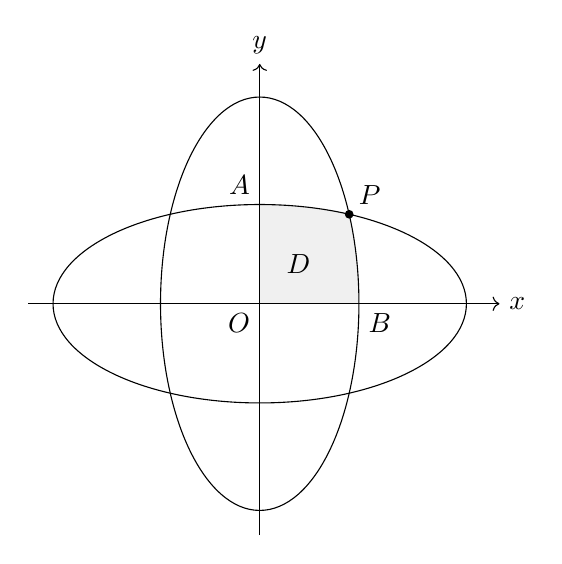
\begin{tikzpicture}[scale=1.05]
\fill[gray!12](0,0)--(1.2,0) arc[start angle=0,end angle=25.64,x radius=1.2,y radius=2.5] arc[start angle=64.36,end angle=90,x radius=2.5,y radius=1.2]--cycle;
\draw(0,0)ellipse(2.5 and 1.2);\draw(0,0)ellipse(1.2 and 2.5);
\draw[->](-2.8,0)--(2.9,0)node[right]{$x$};\draw[->](0,-2.8)--(0,2.9)node[above]{$y$};
\node[below left]at(0,0){$O$};\node[above left]at(0,1.2){$A$};\node[below right]at(1.2,0){$B$};\fill(1.082,1.082)circle(1.5pt)node[above right]{$P$};\node at(.47,.48){$D$};
\end{tikzpicture}\par{\small 图 5.2.5\quad 两椭圆的公共区域（重绘）}
\end{minipage}\end{center}

\entry{例 5.2.12}{含奇点的闭曲线积分（原解存疑）}{p.267}
求
\[
A=\oint_L\frac{x\dd y-y\dd x}{4x^2+y^2},
\]
其中 $L$ 是以 $(1,0)$ 为圆心、$R$ 为半径（$R\ne1$）的圆，取逆时针正向。
\par\textbf{原解（含疑点，见编校注）}\quad 记
\[
P=-\frac y{4x^2+y^2},\quad Q=\frac x{4x^2+y^2},\qquad
Q_x-P_y=\frac{y^2-4x^2}{(4x^2+y^2)^2},\quad (x,y)\ne(0,0).
\]
若 $R<1$，则 $L$ 不包原点，原书由 Green 公式得 $A=0$。

若 $R>1$，则 $L$ 包围原点。取其内部小椭圆
\[
L_1:\quad x=\frac\varepsilon2\cos\theta,\quad y=\varepsilon\sin\theta,\quad0\le\theta\le2\pi.
\]
原书在两曲线所围区域 $D$ 内用 Green 公式，得
\[
A=\oint_{L_1}\frac{x\dd y-y\dd x}{4x^2+y^2}.
\]
作代换，得到
\[
\int_0^{2\pi}\left(\frac12\cos^2\theta+\frac12\sin^2\theta\right)\dd\theta=\pi.
\]
所以原书结论为 $R>1$ 时 $A=\pi$。
\ednote{原书此步 Green 推断与所列旋度不符，题解待核。本稿保留原书所列导数与后续原结论。编校核算：由题面 $P,Q$ 直接求导，应有 $Q_x=P_y=(y^2-4x^2)/(4x^2+y^2)^2$，故原书所印非零表达式并非两者之差。疑点在原书旋度计算与书面论证不一致，不能仅凭此误印断言末答错误；本核算不是原书新增解法。}
\begin{center}\begin{minipage}{\linewidth}\centering
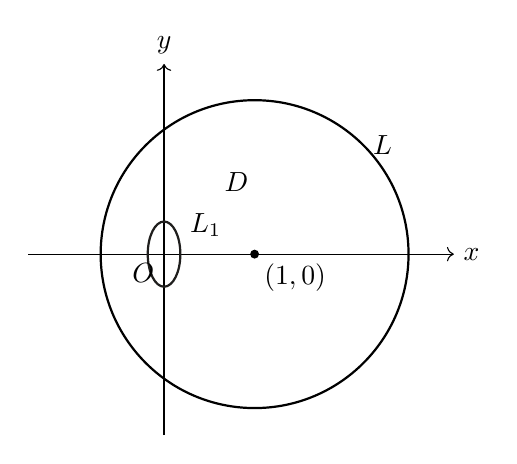
\begin{tikzpicture}[scale=1.15]
\draw[->](-1.5,0)--(3.2,0)node[right]{$x$};\draw[->](0,-2)--(0,2.1)node[above]{$y$};
\draw[thick](1,0)circle(1.7);\draw[thick,navy](0,0)ellipse(.18 and .36);
\fill(1,0)circle(1.4pt)node[below right]{$(1,0)$};\node[below left]at(0,0){$O$};\node[right]at(.18,.32){$L_1$};\node[right]at(2.2,1.2){$L$};\node at(.8,.8){$D$};
\end{tikzpicture}\par{\small 图 5.2.6\quad 外圆与小椭圆（$R>1$ 情形，重绘）}
\end{minipage}\end{center}

\entry{例 5.2.13}{Green 公式证明零边值唯一性}{pp.267—268}
设 $D$ 为 $Oxy$ 平面内有限条逐段光滑曲线围成的区域，$f$ 在 $D$ 上二阶连续，满足
\[
f_{xx}+f_{yy}=2af_x+2bf_y+cf,
\]
其中 $a,b,c$ 为常数，$c\ge0$。证明：若 $f$ 在 $\partial D$ 上恒为零，则在 $D$ 上恒为零。
\prooftext 设 $P=-f(f_y-bf)$、$Q=f(f_x-af)$，则 $P,Q$ 有一阶连续偏导数，且
\begin{align*}
Q_x-P_y&=f_x^2+f_y^2+f(f_{xx}+f_{yy}-2af_x-2bf_y)\\
&=f_x^2+f_y^2+cf^2.
\end{align*}
边界上 $f=0$，从而 $P=Q=0$。由 Green 公式，
\[
0=\oint_{\partial D}P\dd x+Q\dd y
=\iint_D(Q_x-P_y)\dd x\dd y
=\iint_D(f_x^2+f_y^2+cf^2)\dd x\dd y.
\]
因 $c\ge0$，故 $f_x=f_y=0$，$f$ 为常数；再由边界上为零，得 $f$ 在 $D$ 上恒为零。

\entry{例 5.2.14}{带指数系数的零边值问题}{pp.268—269}
设 $D$ 由光滑封闭曲线 $L$ 围成，$f$ 在 $D$ 上二阶连续，满足
\[
e^yf_{xx}+e^xf_{yy}=0,
\]
且在 $L$ 上 $f$ 恒为零。证明：

（1）存在一阶连续的 $P,Q$，满足 $Q_x-P_y=e^y(f_x)^2+e^x(f_y)^2$。

（2）$f$ 在 $D$ 上恒为零。
\prooftext （1）令 $P=-e^xff_y$、$Q=e^yff_x$，则
\begin{align*}
Q_x-P_y&=e^y[(f_x)^2+ff_{xx}]+e^x[(f_y)^2+ff_{yy}]\\
&=e^y(f_x)^2+e^x(f_y)^2+f(e^yf_{xx}+e^xf_{yy})\\
&=e^y(f_x)^2+e^x(f_y)^2.
\end{align*}
（2）因边界上 $P,Q$ 均为零，故 $\oint_LP\dd x+Q\dd y=0$。由 Green 公式，
\[
0=\iint_D[e^y(f_x)^2+e^x(f_y)^2]\dd x\dd y.
\]
被积函数非负，且积分为零，所以 $D$ 上 $f_x=f_y=0$。故 $f$ 为常数，进而恒为零。

\entry{例 5.2.15}{圆盘上函数积分的估计}{p.269}
设 $D:x^2+y^2\le a^2$，$a>0$；$f$ 在 $D$ 上有连续偏导数，边界上 $f=0$。证明
\[
\left|\iint_Df\dd x\dd y\right|\le\frac{\pi a^3}{3}\max_{(x,y)\in D}\sqrt{f_x^2+f_y^2}.
\]
\prooftext 取 $\partial D$ 逆时针方向。由 Green 公式，
\[
\oint_{\partial D}-yf\dd x+xf\dd y=\iint_D(2f+xf_x+yf_y)\dd x\dd y.
\]
左端为零，因此 $2\iint_Df\dd x\dd y=-\iint_D(xf_x+yf_y)\dd x\dd y$。
由 Cauchy 不等式，
\[
|xf_x+yf_y|\le\sqrt{x^2+y^2}\sqrt{f_x^2+f_y^2}.
\]
故
\begin{align*}
2\left|\iint_Df\dd x\dd y\right|
&\le\iint_D\sqrt{x^2+y^2}\sqrt{f_x^2+f_y^2}\dd x\dd y\\
&\le\max_D\sqrt{f_x^2+f_y^2}\iint_D\sqrt{x^2+y^2}\dd x\dd y\\
&=\frac{2\pi a^3}{3}\max_D\sqrt{f_x^2+f_y^2},
\end{align*}
即得所证。

\entry{例 5.2.16}{Poincaré 不等式}{p.270（上半页）}
设 $D$ 为简单光滑闭曲线 $L$ 围成的区域，$f$ 在 $\overline D$ 上有连续偏导数，且 $L$ 上 $f(x,y)=0$。证明
\[
\iint_Df^2(x,y)\dd x\dd y\le\max_D\{x^2+y^2\}\cdot\iint_D[(f_x)^2+(f_y)^2]\dd x\dd y.
\]
\prooftext 记 $M=\max_D\{x^2+y^2\}$。在例 5.2.15 的证明中用 $f^2$ 代替 $f$，得
\[
2\iint_Df^2\dd x\dd y=-\iint_D(2xff_x+2yff_y)\dd x\dd y.
\]
由 Cauchy 积分不等式，
\begin{align*}
\iint_Df^2\dd x\dd y
&\le\iint_D\sqrt{x^2+y^2}\,|f(x,y)|\sqrt{f_x^2+f_y^2}\dd x\dd y\\
&\le\sqrt M\iint_D|f(x,y)|\sqrt{f_x^2+f_y^2}\dd x\dd y\\
&\le\sqrt M\left(\iint_Df^2\dd x\dd y\right)^{1/2}
\left(\iint_D[f_x^2+f_y^2]\dd x\dd y\right)^{1/2},
\end{align*}
由此得证。
\ednote{原书 Cauchy 估计中 $f$ 处应取绝对值，此处补正。}

\clearpage
\section{曲面积分：基本概念及定理}
\src{原书 §5.3，pp.270—273}
\entry{预备结论}{光滑曲面片及面积}{pp.270—271}
设光滑曲面片 $S$ 的参数为
\[
\rr=\rr(u,v)=x(u,v)\vct i+y(u,v)\vct j+z(u,v)\vct k,
\qquad (u,v)\in D,
\]
其中 $x,y,z$ 有连续偏导数，且 $\rr_u\times\rr_v\ne\vct0$。曲面面积为
\[
|S|=\iint_D|\rr_u\times\rr_v|\dd u\dd v.
\]
当曲面写为 $z=f(x,y)$ 时，
\begin{equation}
|S|=\iint_D\sqrt{1+f_x^2+f_y^2}\dd x\dd y.\tag{5.3.1}
\end{equation}

\entry{定义 5.3.1}{第一型曲面积分}{p.271}
设 $S$ 为有界光滑曲面，$f$ 定义于其上。将 $S$ 分为小片 $S_i$，面积记为 $\Delta S_i$，任取介点 $P_i=(\xi_i,\eta_i,\zeta_i)\in S_i$。若极限
\[
\lim_{\lambda\to0}\sum_i f(P_i)\Delta S_i
\]
存在且有限，并与介点选取无关（$\lambda$ 为小片的最大直径），则记为 $\iint_S f(x,y,z)\dd S$，称为第一型曲面积分。

\entry{定理 5.3.1}{第一型曲面积分的计算}{p.271}
设有界光滑曲面 $S$ 具有参数 $\rr(u,v)$，$D$ 为 $Ouv$ 平面内有界闭域，$f$ 在包含 $S$ 的区域内连续，则第一型曲面积分存在，且
\begin{equation}
\iint_S f\dd S=\iint_D f(x(u,v),y(u,v),z(u,v))|\rr_u\times\rr_v|\dd u\dd v,\tag{5.3.2}
\end{equation}
也可写为
\begin{equation}
\iint_S f\dd S=\iint_D f(x(u,v),y(u,v),z(u,v))\sqrt{EG-F^2}\dd u\dd v,\tag{5.3.3}
\end{equation}
其中 $E=|\rr_u|^2$、$G=|\rr_v|^2$、$F=\rr_u\cdot\rr_v$ 为 Gauss 系数。
特别地，若 $S:z=z(x,y)$，则
\[
\iint_S f\dd S=\iint_D f(x,y,z(x,y))\sqrt{1+z_x^2+z_y^2}\dd x\dd y.
\]

\entry{定义 5.3.2}{第二型曲面积分}{pp.271—272}
设 $S$ 为三维向量场 $\FF$ 中的定向光滑曲面，$\nn$ 为单位法向量。将曲面分为面积片，选取介点 $M_i$，若小片最大直径趋于零时，极限
\[
\sum_i\FF(M_i)\cdot\nn(M_i)\Delta S_i
\]
存在，且不依赖于取点，则称为第二型曲面积分，记为
\[
\iint_S\FF\cdot\dd\vct S=\iint_S\FF\cdot\nn\dd S,
\qquad\dd\vct S=\nn\dd S.
\]
这里 $\dd\vct S$ 为有向面积微元。设 $\FF=(P,Q,R)$，$\nn$ 与 $x,y,z$ 轴的夹角分别为 $\alpha,\beta,\gamma$，则
\[
\nn=(\cos\alpha,\cos\beta,\cos\gamma),\quad
\FF\cdot\nn\dd S=P\cos\alpha\dd S+Q\cos\beta\dd S+R\cos\gamma\dd S.
\]
令
\[
\dd y\wedge\dd z=\cos\alpha\dd S,\quad
\dd z\wedge\dd x=\cos\beta\dd S,\quad
\dd x\wedge\dd y=\cos\gamma\dd S,
\]
则
\[
\iint_S\FF\cdot\dd\vct S
=\iint_S[P\dd y\wedge\dd z+Q\dd z\wedge\dd x+R\dd x\wedge\dd y].
\]
记号 $\wedge$ 常略去。

\entry{定理 5.3.2}{第二型曲面积分的参数计算}{p.272}
设 $S$ 的参数为 $\rr=(x(u,v),y(u,v),z(u,v))$，定向为
$\nn=(\rr_u\times\rr_v)/|\rr_u\times\rr_v|$，则
\begin{align*}
\iint_S\FF\cdot\dd\vct S
&=\iint_D\FF\cdot(\rr_u\times\rr_v)\dd u\dd v\\
&=\iint_D\begin{vmatrix}P&Q&R\\x_u&y_u&z_u\\x_v&y_v&z_v\end{vmatrix}\dd u\dd v\\
&=\iint_D\left[P\frac{\partial(y,z)}{\partial(u,v)}+Q\frac{\partial(z,x)}{\partial(u,v)}+R\frac{\partial(x,y)}{\partial(u,v)}\right]\dd u\dd v.
\end{align*}

\entry{定理 5.3.3}{Gauss 公式}{p.272}
设 $V$ 由分片光滑双侧封闭曲面 $S$ 围成，$S$ 取向外方向，$P,Q,R$ 在 $V$ 上有连续一阶偏导数，则
\[
\oiint_{\partial V}P\dd y\dd z+Q\dd z\dd x+R\dd x\dd y
=\iiint_V(P_x+Q_y+R_z)\dd x\dd y\dd z.
\]

\entry{定理 5.3.4}{Stokes 公式}{pp.272—273}
设分片光滑曲面 $S$ 以封闭曲线 $L$ 为边界，$P,Q,R$ 在包含 $S$ 的空间区域内有连续偏导数，则
\begin{align*}
\oint_L P\dd x+Q\dd y+R\dd z
=\iint_S\bigl[&(R_y-Q_z)\dd y\dd z+(P_z-R_x)\dd z\dd x\\
&+(Q_x-P_y)\dd x\dd y\bigr].
\end{align*}
其中 $L$ 的取向与 $S$ 协调，即 $L$ 的方向与曲面法向成右手系。

\clearpage
\section{曲面积分：例题及原解}
\entry{例 5.3.1}{第一卦限球面上的第一型积分}{p.273}
设 $S$ 为第一卦限球面 $x^2+y^2+z^2=R^2$，$x,y,z\ge0$，求 $\iint_S(x^2+y^2)\dd S$。
\sol 由对称性，
\begin{align*}
I&=2\iint_Sx^2\dd S=\frac23\iint_S(x^2+y^2+z^2)\dd S\\
&=\frac{2R^4}{3}\int_0^{\pi/2}\dd\varphi\int_0^{\pi/2}\sin\theta\dd\theta
=\frac{\pi R^4}{3}.
\end{align*}

\entry{例 5.3.2}{柱面所截锥面上的积分}{p.273}
设 $S$ 为锥面 $z^2=k^2(x^2+y^2)$、$z\ge0$ 被柱面 $x^2+y^2=2ax$（$a>0$）所截得的曲面，求 $\iint_S(y^2z^2+z^2x^2+x^2y^2)\dd S$。
\sol 有 $\dd S=\sqrt{1+z_x^2+z_y^2}\dd x\dd y=\sqrt{1+k^2}\dd x\dd y$，投影域为 $D:x^2+y^2\le2ax$。故
\begin{align*}
I&=\sqrt{1+k^2}\iint_D[k^2(x^2+y^2)^2+x^2y^2]\dd x\dd y\\
&=2\sqrt{1+k^2}\int_0^{\pi/2}\dd\varphi\int_0^{2a\cos\varphi}r^5(k^2+\cos^2\varphi\sin^2\varphi)\dd r\\
&=\frac\pi{24}a^6(80k^2+7)\sqrt{1+k^2}.
\end{align*}

\entry{例 5.3.3}{柱侧面上的积分}{p.274}
设 $S$ 为柱面 $x^2+y^2=a^2$ 被 $z=0$、$z=h$（$h>0$）截下的柱面，求 $\iint_S(x^4+y^4)\dd S$。
\sol 取参数 $\rr=(a\cos\varphi,a\sin\varphi,z)$，$0\le\varphi\le2\pi$、$0\le z\le h$。则
\[
\rr_\varphi=(-a\sin\varphi,a\cos\varphi,0),\quad\rr_z=(0,0,1),\quad
|\rr_\varphi\times\rr_z|=a.
\]
由对称性，$\iint_Sx^4\dd S=\iint_Sy^4\dd S$，故
\begin{align*}
I&=2\iint_Sy^4\dd S=2\int_0^h\int_0^{2\pi}a^4\sin^4\varphi\cdot a\dd\varphi\dd z\\
&=8a^5\int_0^{\pi/2}\sin^4\varphi\dd\varphi\cdot\int_0^h\dd z
=\frac32\pi ha^5.
\end{align*}

\entry{例 5.3.4}{球体的平面截面}{pp.274—275}
设 $S(t)$ 为平面 $M(t):x+y+z=t$ 被球 $x^2+y^2+z^2=1$ 截下的部分，$F=1-(x^2+y^2+z^2)$。证明当 $|t|\le\sqrt3$ 时，
\[
\iint_{S(t)}F\dd S=\frac{\pi(3-t^2)^2}{18}.
\]
\prooftext 单位法向量为 $\nn=(1,1,1)/\sqrt3$，原点到平面的距离为 $|t|/\sqrt3$。当 $|t|>\sqrt3$ 时，平面不交球体 $B$；当 $|t|<\sqrt3$ 时，截面为圆盘，中心为 $(t/3,t/3,t/3)$，半径为 $r_0=\sqrt{1-t^2/3}$。
距圆心为 $r$ 的点满足
\[
(x-t/3)^2+(y-t/3)^2+(z-t/3)^2=r^2.
\]
结合 $x+y+z=t$，得 $x^2+y^2+z^2=t^2/3+r^2$。在该平面内取极坐标，$\dd S=r\dd r\dd\varphi$，$(r,\varphi)\in[0,r_0]\times[0,2\pi]$。于是
\begin{align*}
I&=\iint\left[1-\left(\frac{t^2}3+r^2\right)\right]r\dd r\dd\varphi
=2\pi\int_0^{r_0}(r_0^2-r^2)r\dd r\\
&=2\pi\left(\frac{r_0^4}2-\frac{r_0^4}4\right)
=\frac{\pi r_0^4}2=\frac{\pi(3-t^2)^2}{18}.
\end{align*}

\entry{例 5.3.5}{第一型曲面积分的正交变换}{pp.275—276}
设 $S$ 为光滑参数曲面 $\vct X=(x(u,v),y(u,v),z(u,v))$，$D\subset\mathbb R^2$，$f$ 为 $S$ 上连续函数，$\vct A=(a_{ij})$ 为三阶正交矩阵。令 $\widetilde{\vct X}=\vct A\vct X$，将 $S$ 变为 $\widetilde S:\widetilde{\vct X}=\widetilde{\vct X}(u,v)$。证明
\[
\iint_Sf(\vct X)\dd S=\iint_{\widetilde S}f(\vct A^{\mathsf T}\widetilde{\vct X})\dd\widetilde S.
\]
\prooftext 有 $\widetilde{\vct X}_u=\vct A\vct X_u$、$\widetilde{\vct X}_v=\vct A\vct X_v$，且
\begin{align*}
\widetilde E&=|\widetilde{\vct X}_u|^2=\widetilde{\vct X}_u^{\mathsf T}\widetilde{\vct X}_u
=\vct X_u^{\mathsf T}\vct A^{\mathsf T}\vct A\vct X_u
=\vct X_u^{\mathsf T}\vct X_u=|\vct X_u|^2=E,\\
\widetilde G&=G,\\
\widetilde F&=\widetilde{\vct X}_u^{\mathsf T}\widetilde{\vct X}_v
=\vct X_u^{\mathsf T}\vct A^{\mathsf T}\vct A\vct X_v
=\vct X_u^{\mathsf T}\vct X_v=F.
\end{align*}
故 $\widetilde E\widetilde G-\widetilde F^2=EG-F^2$。由第一型积分计算公式，
\begin{align*}
\iint_Sf(\vct X)\dd S
&=\iint_Df(\vct X(u,v))\sqrt{EG-F^2}\dd u\dd v\\
&=\iint_Df(\vct A^{\mathsf T}\widetilde{\vct X}(u,v))\sqrt{\widetilde E\widetilde G-\widetilde F^2}\dd u\dd v\\
&=\iint_{\widetilde S}f(\vct A^{\mathsf T}\widetilde{\vct X})\dd\widetilde S.
\end{align*}

\entry{例 5.3.6}{Poisson 公式}{p.276}
设 $S$ 为单位球面 $x^2+y^2+z^2=1$，$f(t)$ 在 $\mathbb R$ 上连续。证明
\[
\iint_Sf(ax+by+cz)\dd S=2\pi\int_{-1}^1f(kt)\dd t,\qquad k=\sqrt{a^2+b^2+c^2}.
\]
\prooftext $k=0$ 时 $a=b=c=0$，结论显然。设 $k>0$，令 $a_1=a/k$、$b_1=b/k$、$c_1=c/k$。单位向量 $(a_1,b_1,c_1)$ 可补成正交矩阵 $\vct A$，另两行为 $(a_2,b_2,c_2)$、$(a_3,b_3,c_3)$。
变换 $\widetilde{\vct X}=\vct A\vct X$ 使单位球面仍为单位球面 $\widetilde S$。由例 5.3.5，原积分等于 $\iint_{\widetilde S}f(k\widetilde x)\dd\widetilde S$。取
\[
\widetilde x=t,\quad\widetilde y=\sqrt{1-t^2}\sin\varphi,\quad
\widetilde z=\sqrt{1-t^2}\cos\varphi,\quad -1\le t\le1,\quad0\le\varphi\le2\pi.
\]
Gauss 系数为 $E=1/(1-t^2)$、$G=1-t^2$、$F=0$，故
\[
I=\int_{-1}^1\int_0^{2\pi}f(kt)\dd\varphi\dd t=2\pi\int_{-1}^1f(kt)\dd t.
\]
\ednote{末行迭代积分的微分次序按所列上下限规范为 $\dd\varphi\dd t$，不改变原解计算。}

\entry{例 5.3.7}{上半球面的第二型积分}{pp.276—277}
求 $I=\iint_Sx^2\dd y\dd z+y^2\dd z\dd x+z^2\dd x\dd y$，其中 $S$ 为上半球面 $x^2+y^2+z^2=a^2$、$z\ge0$，取上侧。
\sol 取 $x=a\sin\theta\cos\varphi$、$y=a\sin\theta\sin\varphi$、$z=a\cos\theta$，$0\le\theta\le\pi/2$、$0\le\varphi\le2\pi$，则 $\nn=(x,y,z)/a$。故
\begin{align*}
I&=\iint_S(x^2,y^2,z^2)\cdot\frac{(x,y,z)}a\dd S
=\frac1a\iint_S(x^3+y^3+z^3)\dd S\\
&=\frac1a\iint_Sz^3\dd S
=\frac1a\int_0^{2\pi}\int_0^{\pi/2}(a\cos\theta)^3a^2\sin\theta\dd\theta\dd\varphi\\
&=2\pi a^4\int_0^{\pi/2}\cos^3\theta\sin\theta\dd\theta=\frac{\pi a^4}2.
\end{align*}
\textbf{注 5.3.1}\quad 这里利用了奇函数 $x^3,y^3$ 在对称区间上的积分为零。

\entry{例 5.3.8}{上半椭球面的参数计算}{pp.277—278}
求 $I=\iint_Sx^3\dd y\dd z+y^3\dd z\dd x$，其中 $S$ 为上半椭球面 $x^2/a^2+y^2/b^2+z^2/c^2=1$、$z\ge0$，取上侧。
\sol 取参数 $x=a\sin\theta\cos\varphi$、$y=b\sin\theta\sin\varphi$、$z=c\cos\theta$，参数域 $D:0\le\varphi\le2\pi$、$0\le\theta\le\pi/2$。有
\[
\frac{\partial(y,z)}{\partial(\theta,\varphi)}=bc\sin^2\theta\cos\varphi,\quad
\frac{\partial(z,x)}{\partial(\theta,\varphi)}=ac\sin^2\theta\sin\varphi,\quad
\frac{\partial(x,y)}{\partial(\theta,\varphi)}=ab\cos\theta\sin\theta.
\]
$\rr_\theta\times\rr_\varphi$ 指向上侧。因此
\begin{align*}
\iint_Sx^3\dd y\dd z
&=\iint_Da^3\sin^3\theta\cos^3\varphi\cdot bc\sin^2\theta\cos\varphi\dd\theta\dd\varphi\\
&=a^3bc\int_0^{2\pi}\cos^4\varphi\dd\varphi\int_0^{\pi/2}\sin^5\theta\dd\theta
=\frac25\pi a^3bc.
\end{align*}
同理 $\iint_Sy^3\dd z\dd x=(2/5)\pi ab^3c$，合计
\[
I=\frac25\pi abc(a^2+b^2).
\]

\entry{例 5.3.9}{补面为四面体应用 Gauss 公式}{p.278}
求 $A=\iint_Sx\dd y\dd z+y\dd z\dd x+z\dd x\dd y$，其中
$S:\{x,y,z\ge0,\ x+y+z=1\}$，法向量与 $(1,1,1)$ 同向。
\sol 补上三个曲面
\[
\begin{aligned}
S_1&:\{x=0,\ y,z\ge0,\ y+z\le1\},\\
S_2&:\{y=0,\ x,z\ge0,\ x+z\le1\},\\
S_3&:\{z=0,\ x,y\ge0,\ x+y\le1\},
\end{aligned}
\]
组成四面体 $V$，$\partial V$ 取外法向。记 $\omega=x\dd y\dd z+y\dd z\dd x+z\dd x\dd y$。由 Gauss 公式，
\[
\oiint_{\partial V}\omega=\iiint_V3\dd x\dd y\dd z=3\cdot\frac13\cdot\frac12=\frac12.
\]
所以 $A=\frac12-(\iint_{S_1}\omega+\iint_{S_2}\omega+\iint_{S_3}\omega)$。三个补面上的积分均为零，故 $A=1/2$。
\begin{center}\begin{minipage}{\linewidth}\centering
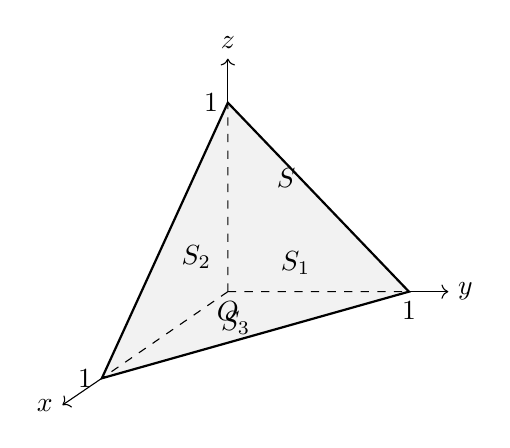
\begin{tikzpicture}[scale=2]
\coordinate(O)at(0,0);\coordinate(X)at(-.8,-.55);\coordinate(Y)at(1.15,0);\coordinate(Z)at(0,1.2);
\fill[gray!10](X)--(Y)--(Z)--cycle;
\draw[dashed](O)--(X)(O)--(Y)(O)--(Z);
\draw[thick](X)--(Y)--(Z)--cycle;
\draw[->](X)--(-1.05,-.72)node[left]{$x$};\draw[->](Y)--(1.4,0)node[right]{$y$};\draw[->](Z)--(0,1.48)node[above]{$z$};
\node[below]at(O){$O$};\node[above right]at(.25,.6){$S$};\node at(.43,.18){$S_1$};\node at(-.2,.22){$S_2$};\node at(.05,-.2){$S_3$};
\node[left]at(X){$1$};\node[below]at(Y){$1$};\node[left]at(Z){$1$};
\end{tikzpicture}\par{\small 图 5.3.1\quad 坐标面四面体与补面（重绘示意）}
\end{minipage}\end{center}
\textbf{注 5.3.2}\quad 当 $S$ 不封闭时，可补上若干光滑曲面，组成封闭曲面来应用 Gauss 公式，前提是补面的积分容易计算。

\entry{例 5.3.10}{平移球体上的 Gauss 公式}{pp.278—279}
求 $A=\iint_Sxy^2\dd y\dd z+yz^2\dd z\dd x+zx^2\dd x\dd y$，其中 $S$ 为球体 $V:\{x^2+y^2+z^2\le z\}$ 的外表面，方向朝外。
\sol 选取球体 $V$ 的参数
\[
x=r\cos\varphi\sin\theta,\quad y=r\sin\varphi\sin\theta,\quad z=\frac12+r\cos\theta,
\]
参数域为 $D:0\le r\le1/2$、$0\le\theta\le\pi$、$0\le\varphi\le2\pi$。由 Gauss 公式，
\begin{align*}
A&=\iiint_V(y^2+z^2+x^2)\dd V\\
&=\iiint_D\left[r^2\sin^2\theta+\frac14+r\cos\theta+r^2\cos^2\theta\right]r^2\sin\theta\dd r\dd\theta\dd\varphi\\
&=2\pi\int_0^\pi\int_0^{1/2}\left(r^2+\frac14+r\cos\theta\right)r^2\sin\theta\dd r\dd\theta\\
&=2\pi\left[\frac15\cdot\frac1{2^5}\cdot2+\frac14\cdot\frac13\cdot\frac1{2^3}\cdot2\right]=\frac\pi{15}.
\end{align*}

\entry{例 5.3.11}{反平方场的通量}{pp.279—280}
求 $I=\iint_S\cos(\rr,\nn)/r^2\dd S$，其中 $S$ 为光滑封闭曲面，原点不在 $S$ 上，$\rr=(x,y,z)$，$r=\sqrt{x^2+y^2+z^2}$，$\nn$ 为外单位法向量。
\sol 因 $\cos(\rr,\nn)=(\rr/r)\cdot\nn$，令
\[
\FF=(P,Q,R)=\left(\frac x{r^3},\frac y{r^3},\frac z{r^3}\right)=\frac{\rr}{r^3},
\]
则 $I=\iint_S\FF\cdot\nn\dd S$。有
\[
P_x=\frac{y^2+z^2-2x^2}{r^5}=\frac1{r^3}-\frac{3x^2}{r^5},\quad
Q_y=\frac1{r^3}-\frac{3y^2}{r^5},\quad R_z=\frac1{r^3}-\frac{3z^2}{r^5},
\]
故三者之和为零。

（1）若原点在 $S$ 外，则 $\FF$ 在其内域 $V$ 中连续可微，由 Gauss 公式，$I=\iiint_V\diver\FF\dd V=0$。

（2）若原点在 $S$ 内，则原点是 $\FF$ 的奇点。取以原点为中心、半径 $\varepsilon$ 的小球面 $S_\varepsilon\subset V$，定向向外。在两面间的夹域内场光滑，故
\[
\iint_{S-S_\varepsilon}\FF\cdot\nn\dd S=0.
\]
于是
\[
I=\iint_{S_\varepsilon}\FF\cdot\nn\dd S
=\iint_{S_\varepsilon}\frac{\rr}{r^3}\cdot\frac{\rr}r\dd S
=\iint_{S_\varepsilon}\frac1{\varepsilon^2}\dd S=4\pi.
\]

\entry{例 5.3.12}{梯度叉积的曲面积分（两解）}{p.280}
设 $S:\{x^2+y^2+z^2=1,\ z>0\}$ 取向上侧，
\[
f(x,y,z)=\frac{1+z}{1+x^2+y^2},\qquad g(x,y,z)=xy+yz+zx.
\]
求 $\iint_S\nabla f\times\nabla g\cdot\dd\vct S$。
\ednote{原书函数变量名写作 $f(x,y),g(x,y)$，但表达式含 $z$；此处补全三变量名。}
\par\textbf{原解·解法一}\quad 直接计算较繁，利用恒等式
\[
\diver(\nabla f\times\nabla g)
=\nabla\cdot(\nabla f\times\nabla g)
=\curl\nabla f\cdot\nabla g-\nabla f\cdot\curl\nabla g=0.
\]
补上底面 $S_1:\{x^2+y^2\le1,z=0\}$，定向与 $z$ 轴正向相反，即 $\nn_1=-\vct k$。由 Gauss 公式，
\[
\oiint_{S\cup S_1}\nabla f\times\nabla g\cdot\dd\vct S
=\iiint_\Omega\diver(\nabla f\times\nabla g)\dd V=0.
\]
所以
\[
\iint_S\nabla f\times\nabla g\cdot\dd\vct S
=-\iint_{S_1}\nabla f\times\nabla g\cdot\dd\vct S
=\iint_{S_1}\nabla f\times\nabla g\cdot\vct k\dd S.
\]
有
\[
\nabla f=\left(-\frac{2x(1+z)}{(1+x^2+y^2)^2},-\frac{2y(1+z)}{(1+x^2+y^2)^2},\frac1{1+x^2+y^2}\right),
\quad\nabla g=(y+z,z+x,x+y).
\]
在 $z=0$ 上，$(\nabla f\times\nabla g)\cdot\vct k=(-2x^2+2y^2)/(1+x^2+y^2)^2$。由对称性，底面积分为
\[
2\iint_{x^2+y^2\le1}\frac{y^2-x^2}{(1+x^2+y^2)^2}\dd x\dd y=0.
\]
\ednote{原书称底面法向与 $z$ 正向相反，却将 $\nn_1$ 印作 $\vct k$；此处明确为 $-\vct k$。}
\par\textbf{原解·解法二}\quad 因 $\nabla f\times\nabla g=\nabla\times(f\nabla g)$，由 Stokes 公式，
\[
\iint_S\nabla f\times\nabla g\cdot\dd\vct S
=\iint_S\nabla\times(f\nabla g)\cdot\dd\vct S
=\oint_{\partial S}f\nabla g\cdot\dd\rr.
\]
边圆 $\partial S:x^2+y^2=1,z=0$ 取协调正向，$f|_{\partial S}=1/2$，且 $\oint_{\partial S}\nabla g\cdot\dd\rr=0$，所以原积分为零。

\entry{例 5.3.13}{调和函数的球面平均值}{p.281}
设 $f$ 在闭球 $B(P_0,R)$ 上二阶连续，且 $\Delta f=f_{xx}+f_{yy}+f_{zz}=0$。证明
\[
f(P_0)=\frac1{4\pi r^2}\iint_Sf\dd S,
\]
其中 $P_0=(x_0,y_0,z_0)$，$S:(x-x_0)^2+(y-y_0)^2+(z-z_0)^2=r^2$，$0\le r\le R$。
\ednote{原书范围含 $r=0$，右端在该点按连续极限解释。}
\prooftext 令 $g(r)$ 为上式右端。取球面参数
\[
x=x_0+r\sin\theta\cos\varphi,\quad y=y_0+r\sin\theta\sin\varphi,\quad z=z_0+r\cos\theta,
\]
其中 $D:0\le\theta\le\pi$、$0\le\varphi\le2\pi$，记 $P$ 为该点。则
\[
g(r)=\frac1{4\pi}\iint_Df(P)\sin\theta\dd\theta\dd\varphi.
\]
记 $B_r=B(P_0,r)$，由 Gauss 公式，
\begin{align*}
g'(r)&=\frac1{4\pi}\iint_D\bigl[\sin\theta\cos\varphi f_x(P)+\sin\theta\sin\varphi f_y(P)\\
&\hspace{43mm}+\cos\theta f_z(P)\bigr]\sin\theta\dd\theta\dd\varphi\\
&=\frac1{4\pi r^2}\iint_S[f_x\dd y\dd z+f_y\dd z\dd x+f_z\dd x\dd y]\\
&=\frac1{4\pi r^2}\iiint_{B_r}\Delta f\dd V=0.
\end{align*}
故 $g$ 为常数，$g(r)=g(0)=f(P_0)$。

\entry{例 5.3.14}{三角形边界上的做功}{pp.281—282}
设 $S:\{x+y+z=1,\ x,y,z\ge0\}$，法向量与 $(1,1,1)$ 同向，$\FF=(y^2,z^2,x^2)$。求绕 $S$ 正向边界 $\partial S$ 一周所做的功。
\sol $\nn=(1,1,1)/\sqrt3$。由 Stokes 公式，
\begin{align*}
W&=\oint_{\partial S}\FF\cdot\dd\rr=\iint_S\curl\FF\cdot\nn\dd S\\
&=\iint_S(-2z,-2x,-2y)\cdot\nn\dd S
=-\frac2{\sqrt3}\iint_S(x+y+z)\dd S\\
&=-\frac2{\sqrt3}\cdot\frac{\sqrt3}{2}=-1.
\end{align*}
\begin{center}\begin{minipage}{\linewidth}\centering
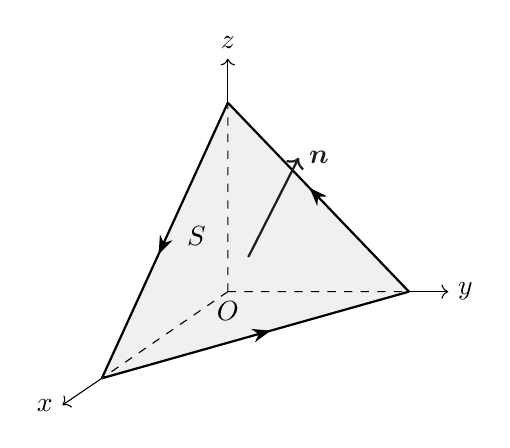
\begin{tikzpicture}[scale=2,midarrow/.style={postaction={decorate},decoration={markings,mark=at position .55 with {\arrow{Stealth}}}}]
\coordinate(O)at(0,0);\coordinate(X)at(-.8,-.55);\coordinate(Y)at(1.15,0);\coordinate(Z)at(0,1.2);
\fill[gray!12](X)--(Y)--(Z)--cycle;
\draw[dashed](O)--(X)(O)--(Y)(O)--(Z);
\draw[thick,midarrow](X)--(Y);\draw[thick,midarrow](Y)--(Z);\draw[thick,midarrow](Z)--(X);
\draw[->](X)--(-1.05,-.72)node[left]{$x$};\draw[->](Y)--(1.4,0)node[right]{$y$};\draw[->](Z)--(0,1.48)node[above]{$z$};
\draw[->,thick,navy](.13,.22)--(.45,.85)node[right]{$\nn$};\node at(-.2,.35){$S$};\node[below]at(O){$O$};
\end{tikzpicture}\par{\small 图 5.3.2\quad 三角面、正向边界与法向（重绘）}
\end{minipage}\end{center}

\entry{例 5.3.15}{椭圆抛物面交线的环量}{p.282}
设 $L$ 为椭圆抛物面 $z=3x^2+4y^2$ 和椭圆柱面 $4x^2+y^2=4y$ 的交线，从 $z$ 轴正向看为顺时针。求 $\FF=(y(z+1),xz,xy-z)$ 沿 $L$ 的环量。
\sol 取 $D:4x^2+y^2\le4y$ 为 $Oxy$ 平面内区域，$S:z=3x^2+4y^2$、$(x,y)\in D$，方向朝下。由 Stokes 公式，
\[
\oint_L\FF\cdot\dd\rr=\iint_S\curl\FF\cdot\dd\vct S
=-\iint_S\dd x\dd y=\iint_D\dd x\dd y=2\pi.
\]
\begin{center}\begin{minipage}{\linewidth}\centering
\begin{tikzpicture}[x={(-.65cm,-.3cm)},y={(.7cm,-.25cm)},z={(0cm,.055cm)},scale=1.05]
\foreach \q in {-.9,-.45,0,.45,.9}{\draw[gray!45,thin]plot[domain=0:4,samples=24,variable=\t]({\q},{\t},{3*\q*\q+4*\t*\t});}
\foreach \q in {.4,1.2,2,2.8,3.6}{\draw[gray!45,thin]plot[domain=-1.1:1.1,samples=18,variable=\t]({\t},{\q},{3*\t*\t+4*\q*\q});}
\draw[dashed]plot[domain=0:360,samples=65,variable=\t]({cos(\t)},{2+2*sin(\t)},0);
\foreach \q in {0,90,180}{\draw[gray!55,dashed]({cos(\q)},{2+2*sin(\q)},0)--({cos(\q)},{2+2*sin(\q)},65);}
\draw[navy,thick]plot[domain=0:360,samples=90,variable=\t]({cos(\t)},{2+2*sin(\t)},{3*cos(\t)*cos(\t)+4*(2+2*sin(\t))^2});
\draw[->](0,0,0)--(1.7,0,0)node[left]{$x$};\draw[->](0,0,0)--(0,4.7,0)node[right]{$y$};\draw[->](0,0,0)--(0,0,75)node[above]{$z$};
\draw[->,thick](0,2,16)--(0,2,3)node[right]{\small 下侧};\node[right]at(0,4,64){$L$};\node[below]at(0,2,0){$D$};
\end{tikzpicture}\par{\small 图 5.3.3\quad 抛物面、柱面交线及下侧（重绘示意，非等比例）}
\end{minipage}\end{center}

\entry{例 5.3.16}{球面与柱面交线的 Stokes 计算}{pp.282—283}
求
\[
I=\oint_L(y^2+z^2)\dd x+(z^2+x^2)\dd y+(x^2+y^2)\dd z,
\]
其中 $L:\{x^2+y^2+z^2=2ax,\ x^2+y^2=2bx,\ z\ge0\}$，$0<b<a$；从 $x$ 轴正向看为逆时针。
\sol 取 $S$ 为 $L$ 在半球面 $x^2+y^2+z^2=2ax$、$z\ge0$ 内围出的面。从 $x$ 轴正向看为逆时针，故 $S$ 的方向朝下，指向球心，
\[
\nn=-\frac{(x-a,y,z)}a.
\]
由 Stokes 公式，
\begin{align*}
I&=2\iint_S(y-z,z-x,x-y)\cdot\nn\dd S\\
&=-2\iint_S(z-y)\dd S=-2\iint_Sz\dd S,
\end{align*}
其中关于 $y$ 的对称性使 $y$ 项积分为零。球面方程给出
\[
z=\sqrt{a^2-(x-a)^2-y^2},\qquad
\dd S=\sqrt{1+z_x^2+z_y^2}\dd x\dd y
=\frac a{\sqrt{a^2-(x-a)^2-y^2}}\dd x\dd y=\frac az\dd x\dd y.
\]
于是
\[
I=-2a\iint_D\dd x\dd y=-2a\pi b^2=-2\pi ab^2,
\qquad D:(x-b)^2+y^2\le b^2.
\]
\ednote{原书此处球面根号中 $y^2$ 前误作正号，面积元分母沿用该误号；此处两处均依球面方程校正为负号。}
\begin{center}\begin{minipage}{\linewidth}\centering
\begin{tikzpicture}[scale=.9]
\begin{scope}
\draw[gray](1.5,1.4)circle(1.4);\draw[gray,dashed](1.5,1.4)ellipse(1.4 and .32);
\draw[dashed](.9,.05)ellipse(.65 and .22);\draw[gray!65](.25,.05)--(.25,2.45)(1.55,.05)--(1.55,2.45);\draw[gray,dashed](.9,2.45)ellipse(.65 and .22);
\draw[navy,thick]plot[smooth]coordinates{(.25,1.4)(.4,2.05)(.85,2.58)(1.35,2.2)(1.55,1.5)(1.15,1.2)(.65,1.12)(.25,1.4)};
\fill(1.5,1.4)circle(1.3pt)node[right]{$(a,0,0)$};\node[left]at(.3,2.15){$L$};\node at(1,-.5){\small 球面与柱面示意};
\end{scope}
\begin{scope}[shift={(5,1.3)}]
\fill[gray!12](.9,0)circle(.9);\draw[thick](.9,0)circle(.9);
\draw[->](-.3,0)--(2.25,0)node[right]{$x$};\draw[->](0,-1.2)--(0,1.3)node[above]{$y$};
\fill(.9,0)circle(1.2pt);\node[below]at(.9,0){$b$};\node[below left]at(0,0){$O$};\node at(.9,.45){$D$};\node at(.9,-1.8){\small 投影圆盘};
\end{scope}
\end{tikzpicture}\par{\small 图 5.3.4\quad 球面、柱面及投影（重绘示意，交线方向见题设）}
\end{minipage}\end{center}

\entry{例 5.3.17}{圆柱斜截椭圆的环量}{p.283}
求
\[
I=\oint_L(y-z)\dd x+(z-x)\dd y+(x-y)\dd z,
\]
其中 $L$ 为柱面 $\Sigma_2:x^2+y^2=a^2$ 与平面 $\pi_1:x/a+z/h=1$（$a,h>0$）的交线，从 $x$ 轴正向看为逆时针。
\sol 取 $S$ 为平面 $\pi_1$ 被柱面截下的部分，$L=\partial S$。其投影为
\[
D_{xy}:x^2+y^2\le a^2,\qquad
D_{yz}:\frac{y^2}{a^2}+\frac{(z-h)^2}{h^2}\le1,
\]
在 $Oxz$ 平面上的投影为直线段。由 Stokes 公式，
\begin{align*}
I&=-2\iint_S[\dd y\dd z+\dd z\dd x+\dd x\dd y]\\
&=-2\iint_{D_{yz}}\dd y\dd z-2\iint_{D_{xy}}\dd x\dd y\\
&=-2\pi ah-2\pi a^2=-2\pi(a+h)a.
\end{align*}
\begin{center}\begin{minipage}{\linewidth}\centering
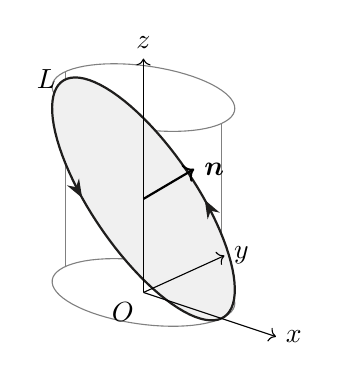
\begin{tikzpicture}[x={(.9cm,-.3cm)},y={(.55cm,.25cm)},z={(0cm,.9cm)},scale=1.1]
\draw[gray]plot[domain=0:360,samples=70,variable=\t]({cos(\t)},{sin(\t)},0);
\draw[gray]plot[domain=0:360,samples=70,variable=\t]({cos(\t)},{sin(\t)},2.5);
\draw[gray](-1,0,0)--(-1,0,2.5)(1,0,0)--(1,0,2.5);
\fill[gray!12]plot[domain=0:360,samples=70,variable=\t]({cos(\t)},{sin(\t)},{1.2*(1-cos(\t))})--cycle;
\draw[thick,navy,postaction={decorate},decoration={markings,mark=at position .2 with {\arrow{Stealth}},mark=at position .7 with {\arrow{Stealth}}}]plot[domain=0:360,samples=90,variable=\t]({cos(\t)},{sin(\t)},{1.2*(1-cos(\t))});
\draw[->](0,0,0)--(1.7,0,0)node[right]{$x$};\draw[->](0,0,0)--(0,1.7,0)node[right]{$y$};\draw[->](0,0,0)--(0,0,3)node[above]{$z$};
\draw[->,thick](0,0,1.2)--(.65,0,1.8)node[right]{$\nn$};\node[left]at(-1,0,2.4){$L$};\node[below left]at(0,0,0){$O$};
\end{tikzpicture}\par{\small 图 5.3.5\quad 圆柱与斜截椭圆的协调取向（重绘）}
\end{minipage}\end{center}

\entry{例 5.3.18}{球面大圆上的线性场积分}{pp.283—284（上半页）}
设 $a,b,c$ 不全为零，$L$ 为球面 $S:x^2+y^2+z^2=R^2$（$R>0$）与平面 $\Sigma:ax+by+cz=0$ 的交线，$L$ 的正向与平面法向量 $(a,b,c)$ 成右手系。求
\[
I=\oint_L(bz+c)\dd x+(cx+a)\dd y+(ay+b)\dd z.
\]
\sol 球体与平面截得大圆盘 $D$，其单位法向量为
\[
\nn=\frac{(a,b,c)}{\sqrt{a^2+b^2+c^2}},
\]
$L$ 为 $D$ 的边界。由 Stokes 公式，
\begin{align*}
I&=\iint_D\curl(bz+c,cx+a,ay+b)\cdot\nn\dd S\\
&=\iint_D(a,b,c)\cdot\nn\dd S
=\sqrt{a^2+b^2+c^2}\iint_D\dd S\\
&=\sqrt{a^2+b^2+c^2}\,\pi R^2.
\end{align*}

\clearpage
\section{相关真题：曲线积分与曲面积分}
\src{§5.4，pp.296—297}
本节为筛选摘录。原书例 5.4.1—5.4.14 为纯 Riemann 积分、函数与积分不等式等（包括例 5.4.11 的纯二重积分），均不收入；此处仅收例 5.4.15、5.4.16。

\entry{例 5.4.15}{第九届全国决赛题}{pp.296—297}
求第二型曲线积分
\[
I=\int_\Gamma e^{\sin x}(\cos x\cos y\dd x-\sin y\dd y)+\cos z\dd z,
\]
其中 $\Gamma:x=\pi\sin(t/2)$、$y=t-\sin t$、$z=\sin2t$，$0\le t\le\pi$。
\sol 记 $P=e^{\sin x}\cos x\cos y$、$Q=-e^{\sin x}\sin y$、$R=\cos z$，则 $P,Q,R$ 在 $\mathbb R^3$ 上连续可微，且
\[
\rot(P,Q,R)=(R_y-Q_z,P_z-R_x,Q_x-P_y)=(0,0,0),
\]
故积分仅与端点有关。$\Gamma$ 的端点为 $(0,0,0)$、$(\pi,\pi,0)$，因此
\begin{align*}
I&=\int_{(0,0,0)}^{(\pi,\pi,0)}P\dd x+Q\dd y+R\dd z\\
&=\int_{(0,0,0)}^{(\pi,0,0)}P\dd x+Q\dd y+R\dd z
+\int_{(\pi,0,0)}^{(\pi,\pi,0)}P\dd x+Q\dd y+R\dd z\\
&=\int_0^\pi e^{\sin x}\cos x\dd x+\int_0^\pi(-\sin y)\dd y=0-2=-2.
\end{align*}
\ednote{原解 $P$ 漏 $\cos x$、$Q$ 漏负号及折线路径首项符号已依题面和方向校正；不改变原解法及末答。}

\entry{例 5.4.16}{第八届全国决赛题}{p.297}
求
\[
I=\iint_S\frac{ax\dd y\dd z+(z+a)^2\dd x\dd y}{\sqrt{x^2+y^2+z^2}},
\]
其中 $a>0$ 为常数，$S:z=-\sqrt{a^2-x^2-y^2}$，取向上侧。
\sol 在 $S$ 上 $x^2+y^2+z^2=a^2$，所以
\[
I=\frac1a\iint_S[ax\dd y\dd z+(z+a)^2\dd x\dd y].
\]
补底 $D:\{x^2+y^2\le a^2,z=0\}$，取向上侧，则 $S^{-1}\cup D$ 为闭下半球体 $B$ 的表面，取向外侧。由 Gauss 公式，
\begin{align*}
&\oiint_{S^{-1}\cup D}[ax\dd y\dd z+(z+a)^2\dd x\dd y]\\
&\quad=\iiint_B(3a+2z)\dd V\\
&\quad=3a\cdot\frac{2\pi a^3}{3}
+2\int_0^{2\pi}\int_{\pi/2}^\pi\int_0^a(r\cos\theta)r^2\sin\theta\dd r\dd\theta\dd\varphi\\
&\quad=2\pi a^4-\frac{\pi a^4}{2}=\frac{3\pi a^4}{2}.
\end{align*}
所以
\begin{align*}
\iint_S[ax\dd y\dd z+(z+a)^2\dd x\dd y]
&=-\frac{3\pi a^4}{2}+\iint_D[ax\dd y\dd z+(z+a)^2\dd x\dd y]\\
&=-\frac{3\pi a^4}{2}+\iint_Da^2\dd x\dd y\\
&=-\frac{3\pi a^4}{2}+\pi a^4=-\frac{\pi a^4}{2}.
\end{align*}
故 $I=-\pi a^3/2$。
\ednote{原书补面 $D$ 仅写 $x^2+y^2=a^2$；此处依 Gauss 公式的应用，明确为 $z=0$ 上的闭圆盘。}

\clearpage
\section{反常积分：无穷区间上的积分}
\src{原书 §6.1，pp.298—309（上半页）}
\entry{定义 6.1.1}{无穷区间积分及收敛类型}{p.298}
设 $f$ 定义在 $[a,+\infty)$ 上，在任意有限区间 $[a,A]$ 上可积。如果 $\varphi(A)=\int_a^Af(x)\dd x$ 在 $A\to+\infty$ 时有有限极限，则定义
\[
\int_a^\infty f(x)\dd x=\lim_{A\to+\infty}\int_a^Af(x)\dd x=\lim_{A\to+\infty}\varphi(A),
\]
称积分存在或收敛，否则称不存在或发散。若 $\int_a^\infty f$ 收敛而 $\int_a^\infty|f|$ 发散，称为条件收敛；若 $\int_a^\infty|f|$ 收敛，称为绝对收敛。类似地，
\[
\int_{-\infty}^af(x)\dd x=\lim_{c\to-\infty}\int_c^af(x)\dd x.
\]
整轴积分定义为
\[
\int_{-\infty}^\infty f(x)\dd x=\int_{-\infty}^af(x)\dd x+\int_a^\infty f(x)\dd x,
\]
须左右两项分别收敛；分点 $a$ 任意，通常取 $0$。

\entry{定理 6.1.1}{类 Newton--Leibniz 公式}{p.299}
设 $f$ 在 $[a,+\infty)$ 上的无穷积分收敛，且有原函数 $F$，则
\[
\int_a^\infty f(x)\dd x=F(+\infty)-F(a).
\]
在 $(-\infty,a]$ 上时，积分为 $F(a)-F(-\infty)$；在全轴上时，为 $F(+\infty)-F(-\infty)$。

\entry{命题 6.1.2}{线性}{p.299}
若 $f,g$ 在 $[a,\infty)$ 上的无穷积分收敛，则对任意 $c_1,c_2$，
\[
\int_a^\infty(c_1f+c_2g)\dd x=c_1\int_a^\infty f\dd x+c_2\int_a^\infty g\dd x.
\]

\entry{命题 6.1.3}{换元公式}{p.299}
设 $f$ 的积分收敛，$\varphi$ 为 $[\alpha,\beta)$（$\beta$ 可为 $+\infty$）上连续可微且严格单调递增的函数，满足 $\varphi(\alpha)=a$、$\lim_{t\to\beta^-}\varphi(t)=\infty$，则
\[
\int_a^\infty f(x)\dd x=\int_\alpha^\beta f(\varphi(t))\varphi'(t)\dd t.
\]

\entry{命题 6.1.4}{分部积分公式}{p.299}
设 $u,v$ 在 $[a,\infty)$ 上连续可微，且 $\lim_{x\to\infty}u(x)v(x)$ 存在。若 $uv'$、$u'v$ 中一个的无穷积分收敛，则另一个也收敛，且
\[
\int_a^\infty uv'\dd x=[uv]_a^\infty-\int_a^\infty u'v\dd x.
\]
\textbf{注 6.1.1}\quad 广义分部积分公式在形式上与常义积分相同，既可计算已知收敛的积分，也可用于证明收敛。

\entry{定理 6.1.5}{Cauchy 准则}{p.299}
设 $f$ 在任意有限区间 $[a,b]$ 上可积。$\int_a^\infty f$ 收敛的充要条件是：任意 $\varepsilon>0$，存在 $B>a$，使 $b_1,b_2>B$ 时
\[
|F(b_2)-F(b_1)|=\left|\int_{b_1}^{b_2}f(x)\dd x\right|<\varepsilon.
\]

\entry{定理 6.1.6}{非负函数积分的有界性判据}{p.300}
设 $f\ge0$，且在任意有限子区间上可积。$\int_a^\infty f$ 收敛的充要条件是：存在 $M>0$，使任意 $b>a$ 均有 $\int_a^bf(x)\dd x<M$，即积分上限函数 $F(b)$ 有界。

\entry{定理 6.1.7}{绝对收敛蕴含收敛}{p.300}
设 $f$ 在任意有限子区间上可积。如果 $\int_a^\infty|f|$ 收敛，则 $\int_a^\infty f$ 收敛。

\entry{定理 6.1.8}{比较判别法}{p.300}
设 $f,g$ 定义于 $[a,\infty)$，在各有限子区间上可积，充分大的 $x$ 满足 $0\le f(x)\le g(x)$。若 $\int_a^\infty g$ 收敛，则 $\int_a^\infty f$ 收敛。

\entry{定理 6.1.9}{Cauchy 判别法}{p.300}
若 $f$ 在 $[1,\infty)$ 上非负且单调递减，则 $\int_1^\infty f(x)\dd x$ 与 $\sum_{n=1}^\infty f(n)$ 同敛散。

\entry{定理 6.1.10}{比较极限判别法}{p.300}
设 $f,g\ge0$，在各有限子区间上可积，且 $\lim_{x\to\infty}f(x)/g(x)=k$。

当 $0<k<\infty$ 时，两积分同敛散；当 $k=0$ 时，$\int_a^\infty g$ 收敛蕴含 $\int_a^\infty f$ 收敛；当 $k=\infty$ 时，$\int_a^\infty g$ 发散蕴含 $\int_a^\infty f$ 发散。

\entry{定理 6.1.11}{Dirichlet 判别法}{p.300}
若 $F(b)=\int_a^bf(x)\dd x$ 作为 $b$ 的函数在 $(a,\infty)$ 上有界，$g$ 在 $(a,\infty)$ 上单调且趋于零，则 $\int_a^\infty fg\dd x$ 收敛。

\entry{定理 6.1.12}{Abel 判别法}{p.301}
若 $\int_a^\infty f$ 收敛，$g$ 在 $[a,\infty)$ 上单调有界，则 $\int_a^\infty fg\dd x$ 收敛。

\entry{例 6.1.1}{收敛积分与函数趋零}{pp.301—302}
（1）若 $f$ 在 $[0,\infty)$ 上连续且 $\int_0^\infty f$ 收敛，则存在正数列 $x_n\to\infty$，使 $f(x_n)\to0$。

（2）若 $f$ 还一致连续，则 $\lim_{x\to\infty}f(x)=0$。
\prooftext （1）对每个正整数 $n$，由积分中值定理存在 $x_n\in(n,n+1)$，使
\[
\int_n^{n+1}f(x)\dd x=f(x_n).
\]
因为积分收敛，
\[
\lim_{n\to\infty}\int_n^{n+1}f
=\lim_{n\to\infty}\left(\int_0^{n+1}f-\int_0^nf\right)=0.
\]
（2）反证。若 $f$ 不趋于零，则存在 $\varepsilon>0$ 和严格递增的 $x_n\to\infty$，使 $|f(x_n)|\ge\varepsilon$；不妨设 $f(x_n)\ge\varepsilon$。由一致连续性，存在 $\delta>0$，使 $|x-y|\le\delta$ 时 $|f(x)-f(y)|<\varepsilon/2$。当 $x_n\le x\le x_n+\delta$ 时，
\[
f(x)=f(x_n)+f(x)-f(x_n)\ge f(x_n)-|f(x)-f(x_n)|\ge\frac\varepsilon2.
\]
故 $\int_{x_n}^{x_n+\delta}f\ge\delta\varepsilon/2$。但收敛积分在这些尾区间上的积分应趋于零，矛盾。

\entry{例 6.1.2}{Young 不等式与收敛性}{p.302}
设 $0<\alpha\le1$、$\beta>0$、$\alpha+\beta>1$，$f$ 为 $[1,\infty)$ 上正函数，且 $\int_1^\infty f$ 收敛。证明 $\int_1^\infty(f(x))^\alpha/x^\beta\dd x$ 收敛。
\prooftext $\alpha=1$ 时由比较判别法即得。设 $\alpha<1$，由 Young 不等式，
\[
(f(x))^\alpha\left(\frac1{x^{\beta/(1-\alpha)}}\right)^{1-\alpha}
\le\alpha f(x)+\frac{1-\alpha}{x^{\beta/(1-\alpha)}}.
\]
因 $\alpha+\beta>1$，故 $\beta/(1-\alpha)>1$，右端幂函数的无穷积分收敛，由此得证。

\entry{例 6.1.3}{仅一次幂可积的正函数}{pp.302—303}
证明存在 $[0,\infty)$ 上的正函数 $f$，使 $\int_0^\infty f$ 收敛，但对任意正数 $p\ne1$，$\int_0^\infty f^p$ 发散。
\prooftext $p<1$ 时令 $\beta=p$；$p>1$ 时令 $\beta=2-p$，原书称“总有 $0<\beta<1$”。取 $0<a_n<1/2$，使 $\sum a_n=a<\infty$ 而 $\sum a_n^\beta=\infty$，例如
\[
a_n=\frac1{n(\ln(n+4))^2}.
\]
当 $x\in[n-1,n)$ 时定义
\[
f(x)=\begin{cases}
a_n,&n-1\le x<n-a_n^2,\\
1/a_n,&n-a_n^2\le x<n.
\end{cases}
\]
则 $\int_{n-1}^nf=a_n(1-a_n^2)+a_n<2a_n$，因此 $\int_0^\infty f$ 收敛。又
\[
\int_{n-1}^nf^p=a_n^p(1-a_n^2)+a_n^{2-p}
>\frac12a_n^p+a_n^{2-p}>\frac12a_n^\beta,
\]
所以积分发散。
\ednote{原书“总有 $0<\beta<1$”的说法在 $p>1$ 一侧仅对 $1<p<2$ 成立。$p\ge2$ 时，可由高峰项 $a_n^{2-p}$ 不趋于零直接判定发散。这是原证的范围疏漏，不改变题面结论；本注的补充不冒充原解。}

\entry{例 6.1.4}{指数衰减控制任意幂}{p.303}
证明对任意实数 $\alpha$，$\int_1^\infty x^\alpha e^{-x}\dd x$ 收敛。
\prooftext 因 $\lim_{x\to\infty}x^\alpha e^{-x/2}=0$，充分大的 $x$ 满足
\[
x^\alpha e^{-x}=x^\alpha e^{-x/2}e^{-x/2}<e^{-x/2}.
\]
后者的积分收敛，由比较判别法得证。

\entry{例 6.1.5}{比较极限法的应用}{p.303}
证明 $\int_1^\infty\dfrac{x^2}{\sqrt{x+1}(x^4+x+1)}\dd x$ 收敛。
\prooftext 当 $x\to\infty$ 时，
\[
\frac{x^2}{\sqrt{x+1}(x^4+x+1)}\sim\frac1{x^{5/2}}.
\]
右端幂函数的积分收敛，由比较极限判别法得证。

\entry{例 6.1.6}{导数绝对可积给出的点态估计}{pp.303—304}
设 $f$ 在 $[0,\infty)$ 上连续可微，$\int_0^\infty f(t)\dd t$ 与 $\int_0^\infty|f'(t)|\dd t$ 均收敛。证明
\[
|f(x)|\le\int_x^\infty|f'(t)|\dd t.
\]
\prooftext 因 $\int_0^\infty|f'|$ 收敛，由 Cauchy 准则，任意 $\varepsilon>0$，存在 $A>0$，使 $y>x>A$ 时 $\int_x^y|f'|<\varepsilon$。由 Newton--Leibniz 公式，
\[
|f(y)-f(x)|=\left|\int_x^yf'(t)\dd t\right|\le\int_x^y|f'(t)|\dd t<\varepsilon.
\]
由 Cauchy 准则，$\lim_{x\to\infty}f(x)=c$ 存在。若 $c\ne0$，不妨设 $c>0$，则充分大的 $t>A$ 满足 $f(t)>c/2$，从而
\[
\int_A^xf(t)\dd t\ge\frac c2(x-A)\to\infty,
\]
与 $\int_0^\infty f$ 收敛矛盾，故 $c=0$。在 $|f(y)-f(x)|\le\int_x^y|f'|$ 中令 $y\to\infty$，即得所证。

\entry{例 6.1.7}{积分不等式及最佳系数}{pp.304—305}
设 $f$ 为 $[0,\infty)$ 上正连续函数，$\int_0^\infty1/f(x)\dd x$ 收敛，$F(x)=\int_0^xf(t)\dd t$。证明
\[
\int_0^\infty\frac{x}{F(x)}\dd x<2\int_0^\infty\frac1{f(x)}\dd x,
\]
且系数 $2$ 最佳。
\prooftext 当 $x>0$ 时，由 Cauchy 积分不等式，
\[
\frac{x^2}{2}=\int_0^xt\dd t
=\int_0^x\sqrt{f(t)}\frac{t}{\sqrt{f(t)}}\dd t
\le\left(\int_0^xf\right)^{1/2}\left(\int_0^x\frac{t^2}{f(t)}\dd t\right)^{1/2}.
\]
所以 $x/F(x)\le(4/x^3)\int_0^xt^2/f(t)\dd t$。等号仅在 $f(t)=ct$ 时成立，但此时 $\int_0^\infty1/f$ 发散，故原书写作严格不等式
\[
\frac{x}{F(x)}<\frac4{x^3}\int_0^x\frac{t^2}{f(t)}\dd t.
\]
两端对 $x$ 从 $0$ 到 $\infty$ 积分，得
\begin{align*}
\int_0^\infty\frac{x}{F(x)}\dd x
&<4\int_0^\infty\left[\frac1{x^3}\int_0^x\frac{t^2}{f(t)}\dd t\right]\dd x\\
&=4\int_0^\infty\left[\int_t^\infty\frac{t^2}{x^3f(t)}\dd x\right]\dd t
=2\int_0^\infty\frac1{f(t)}\dd t.
\end{align*}
为证最优性，取 $f_p(x)=(x+a)^p$，$a=p-1>0$，则
\[
\int_0^\infty\frac1{f_p(x)}\dd x=\frac1{(p-1)a^{p-1}},\qquad
F(x)=\frac{(x+a)^{p+1}-a^{p+1}}{p+1}.
\]
因此
\[
\int_0^\infty\frac{x}{F(x)}\dd x
=(p+1)\int_0^\infty\frac{x}{(x+a)^{p+1}-a^{p+1}}\dd x.
\]
原书称不难证明，对 $x>0$、$p\ge1$，有
\[
\frac{x}{(x+a)^{p+1}-a^{p+1}}\ge\frac1{p(x+2a)^p}.
\]
由此
\begin{align*}
\int_0^\infty\frac{x}{F(x)}\dd x
&\ge\frac{p+1}{p}\int_0^\infty\frac1{(x+2a)^p}\dd x\\
&=\frac{(p+1)/p}{(p-1)(2a)^{p-1}}
=\frac{p+1}{p\,2^{p-1}}\int_0^\infty\frac1{f_p(x)}\dd x.
\end{align*}
当 $p\to1^+$ 时，$(p+1)/(p\,2^{p-1})\to2$，故系数最佳。

\entry{注 6.1.1（原编号）}{Hölder 推广}{pp.305—306}
由 Hölder 不等式可得更一般结果：设 $\alpha>0$，$f$ 为正连续函数，$\int_0^\infty1/(f(x))^\alpha\dd x$ 收敛，$F(x)=\int_0^xf(t)\dd t$，则
\[
\int_0^\infty\left(\frac{x}{F(x)}\right)^\alpha\dd x
<\left(\frac{1+\alpha}{\alpha}\right)^\alpha\int_0^\infty\frac1{(f(x))^\alpha}\dd x,
\]
且系数 $((1+\alpha)/\alpha)^\alpha$ 最佳。
\ednote{原书此注与 p.299 的“注 6.1.1”重号，本稿保留原编号并以出处区分。}

\entry{例 6.1.8}{Dirichlet 积分}{pp.306—307}
求 $\int_0^\infty(\sin x)/x\dd x$。
\sol 将恒等式
\[
\frac12+\cos x+\cos2x+\cdots+\cos nx
=\frac{\sin((n+1/2)x)}{2\sin(x/2)}
\]
在 $[0,\pi]$ 上积分，得
\begin{equation}
\int_0^\pi\frac{\sin((n+1/2)x)}{2\sin(x/2)}\dd x=\frac\pi2.\tag{6.1.1}
\end{equation}
令
\[
\varphi(x)=\frac1x-\frac1{2\sin(x/2)}
=\frac{2\sin(x/2)-x}{2x\sin(x/2)},\quad0<x\le\pi.
\]
由 $\lim_{x\to0}\varphi(x)=0$，补充 $\varphi(0)=0$ 后连续。由 Riemann--Lebesgue 引理，
\[
\lim_{k\to\infty}\int_0^\pi\varphi(x)\sin(kx)\dd x=0.
\]
取 $k=n+1/2$，结合式（6.1.1），得
\[
\lim_{n\to\infty}\int_0^\pi\frac{\sin((n+1/2)x)}x\dd x=\frac\pi2.
\]
换元 $u=(n+1/2)x$，即有
\[
\lim_{n\to\infty}\int_0^{(n+1/2)\pi}\frac{\sin u}u\dd u=\frac\pi2,
\qquad\int_0^\infty\frac{\sin x}x\dd x=\frac\pi2.
\]
\ednote{收敛性由 Dirichlet 判别法保证；此句为编校交叉提示。}

\entry{例 6.1.9}{连乘分母的积分}{p.307}
求 $\int_1^\infty\dd x/[x(x+1)\cdots(x+n)]$，其中 $n$ 为正整数。
\sol 部分分式分解为
\[
\frac1{x(x+1)\cdots(x+n)}=\frac{a_0}x+\frac{a_1}{x+1}+\cdots+\frac{a_n}{x+n}.
\]
两端乘 $x+k$ 再令 $x=-k$，得 $a_k=((-1)^k/n!)\binom nk$，$k=0,\ldots,n$。原函数为
$F(x)=\sum_{k=0}^na_k\ln(x+k)$。因
\[
\sum_{k=0}^na_k=\frac1{n!}\sum_{k=0}^n(-1)^k\binom nk=0,
\]
故
\[
F(x)=\sum_{k=0}^na_k[\ln(x+k)-\ln x]=\sum_{k=0}^na_k\ln(1+k/x),\quad F(+\infty)=0.
\]
所求积分为
\[
F(+\infty)-F(1)=\sum_{k=0}^n\frac{(-1)^{k+1}}{n!}\binom nk\ln(1+k).
\]

\entry{例 6.1.10}{含幂变换的极限}{pp.307—308}
设 $a>1$，$f$ 在 $[1,\infty)$ 上连续，$\lim_{x\to\infty}xf(x)$ 存在且有限。证明 $\int_1^\infty f(x)/x\dd x$ 收敛，且
\[
\lim_{n\to\infty}n\int_1^af(x^n)\dd x=\int_1^\infty\frac{f(x)}x\dd x.
\]
\prooftext 存在 $M>0$，使 $|xf(x)|\le M$（$x\ge1$），从而 $|f(x)/x|\le M/x^2$，故积分绝对收敛。令 $t=x^n$，有
\[
n\int_1^af(x^n)\dd x=\int_1^{a^n}\frac{f(t)}t\,t^{1/n}\dd t.
\]
由于 $\int_1^{a^n}f(t)/t\dd t\to\int_1^\infty f(x)/x\dd x$，只须证明
\begin{equation}
\lim_{n\to\infty}\int_1^{a^n}\frac{f(t)}t(t^{1/n}-1)\dd t=0.\tag{6.1.2}
\end{equation}
任意 $\varepsilon>0$，取 $A>1$，使 $M(a-1)/A<\varepsilon$；再取 $N$，使 $n>N$ 时 $a^n>A$，且 $M(A-1)(A^{1/n}-1)<\varepsilon$。此时将绝对值分为 $[1,A]$ 与 $[A,a^n]$ 两段，得
\[
\left|\int_1^{a^n}\frac{f(t)}t(t^{1/n}-1)\dd t\right|
\le M(A-1)(A^{1/n}-1)+\frac{M(a-1)}A<2\varepsilon.
\]
由此得证。

\entry{例 6.1.11}{正导数函数的不等式}{pp.308—309（上半页）}
设 $f$ 在 $\mathbb R$ 上三阶连续可微，$f$ 及各阶导数恒正，且 $f'''\le f$。证明对任意 $x$ 有
\[
\text{（i）}\quad\frac12(f''(x))^2+\int_{-\infty}^x(f'(t))^2\dd t\le f(x)f'(x);
\]
\[
\text{（ii）}\quad f'(x)<\left(\frac43\right)^{1/3}f(x).
\]
\prooftext （i）$f,f',f''$ 严格递增，$\lim_{x\to-\infty}f(x)$ 存在。由微分中值定理，存在 $\theta_x\in(x,x+1)$，使
\[
f(x+1)-f(x)=f'(\theta_x)>f'(x)>0.
\]
因此 $\lim_{x\to-\infty}f'(x)=0$。同理 $\lim_{x\to-\infty}f''(x)=0$。由 $f'''\le f$，得
\[
f''f'''+(f')^2\le ff''+(f')^2.
\]
在 $(-\infty,x]$ 上积分，便得（i）。

（ii）由 $f''$ 递增，
\[
\int_{-\infty}^x(f')^2\dd t
\ge\frac1{f''(x)}\int_{-\infty}^x(f')^2f''\dd t
=\frac{(f'(x))^3}{3f''(x)}.
\]
所以 $\frac12(f'')^2+(f')^3/(3f'')\le ff'$。将左端拆分，由均值不等式，原书写为
\begin{align*}
\frac14(f'')^2+\frac14(f'')^2+\frac{(f')^3}{3f''}
&\ge3\left[\frac14(f'')^2\cdot\frac14(f'')^2\cdot\frac{(f')^3}{3f''}\right]^{1/3}\\
&=\left(\frac34\right)^{2/3}f'f''.
\end{align*}
于是 $f''\le(4/3)^{2/3}f$。两端乘 $f'$，在 $(-\infty,x]$ 上积分，可得（ii）。
\ednote{原书最后一步仅概述“积分得结论”，此处保留该篇幅；严格不等号及无穷端常数的论证未在原解中展开。}

\clearpage
\section{反常积分：瑕积分}
\src{原书 §6.2，pp.309（下半页）—312（上半页）}
\entry{定义 6.2.1}{端点瑕积分}{p.309}
设 $f$ 定义于 $(a,b]$，$a$ 为瑕点，原书以 $\lim_{x\to a^+}f(x)=+\infty$ 的端点型情形说明。若内部任意闭区间上可积，则定义
\[
\int_a^bf(x)\dd x=\lim_{\varepsilon\to0^+}\int_{a+\varepsilon}^bf(x)\dd x.
\]
极限有限时称为收敛。右端点为瑕点的情形类似。作换元 $y=1/(x-a)$，有
\[
\int_a^bf(x)\dd x=\int_{1/(b-a)}^\infty\frac{f(a+1/y)}{y^2}\dd y.
\]
因此，瑕积分可转为无穷区间广义积分，相应判别法同样成立。

\entry{定理 6.2.1}{Cauchy 准则}{p.310}
设 $f$ 定义于 $(a,b]$，$a$ 为唯一瑕点。$\int_a^bf$ 收敛的充要条件是：任意 $\varepsilon>0$，存在 $\delta>0$，使 $0<\delta',\delta''<\delta$ 时
\[
\left|\int_{a+\delta'}^{a+\delta''}f(x)\dd x\right|<\varepsilon.
\]

\entry{定理 6.2.2}{绝对收敛蕴含收敛}{p.310}
在上述条件下，若 $\int_a^b|f|$ 收敛，则 $\int_a^bf$ 收敛。

\entry{定理 6.2.3}{比较判别法}{p.310}
设 $a$ 为唯一瑕点，充分靠近 $a$ 的 $x>a$ 满足 $0\le f(x)\le g(x)$。则：

（1）$\int_a^bg$ 收敛蕴含 $\int_a^bf$ 收敛。

（2）$\int_a^bf$ 发散蕴含 $\int_a^bg$ 发散。

\entry{定理 6.2.4}{比较极限判别法}{p.310}
设 $f,g$ 在 $(a,b]$ 上非负连续，$a$ 为唯一瑕点，$\lim_{x\to a^+}f(x)/g(x)=k$。

当 $0<k<\infty$ 时，两积分同敛散；当 $k=0$ 且 $\int_a^bg$ 收敛时，$\int_a^bf$ 收敛；当 $k=\infty$ 且 $\int_a^bg$ 发散时，$\int_a^bf$ 发散。

\entry{例 6.2.1}{椭圆积分的收敛性}{pp.310—311}
研究 $\int_0^1\dd x/\sqrt{(1-x^2)(1-k^2x^2)}$ 的敛散性，其中 $0<k<1$。
\sol $x=1$ 为瑕点，且
\[
\lim_{x\to1^-}\frac{1/\sqrt{(1-x^2)(1-k^2x^2)}}{1/\sqrt{1-x}}
=\frac1{\sqrt{2(1-k^2)}}.
\]
因 $\int_0^1\dd x/\sqrt{1-x}$ 收敛，由比较极限判别法知原积分收敛。

\entry{例 6.2.2}{对数型瑕积分}{p.311}
研究 $\int_0^1\ln x/(1-x^2)\dd x$ 的敛散性。
\sol 看似 $x=0,1$ 都是瑕点，但 $\lim_{x\to1}\ln x/(1-x^2)=-1/2$，故 $1$ 为可去瑕点。充分小的 $x$ 满足 $1-x^2\ge1/2$，则
\[
\left|\frac{\ln x}{1-x^2}\right|\le2|\ln x|.
\]
而
\[
\int_0^1|\ln x|\dd x=-\int_0^1\ln x\dd x
=-[x\ln x]_0^1+\int_0^1\dd x=1
\]
收敛，故原积分收敛。

\entry{例 6.2.3}{同时含瑕点与无穷上限}{p.311}
研究 $\int_0^\infty x^\alpha\arctan x/(2+x^\beta)\dd x$ 的敛散性，其中 $\beta\ge0$。
\sol $\alpha<0$ 时 $x=0$ 为瑕点，又有无穷上限，故拆为 $\int_0^1+\int_1^\infty$。当 $x\to0^+$ 时，原书写为
\[
\frac{x^\alpha\arctan x}{2+x^\beta}\sim\frac12x^{\alpha+1}.
\]
因此 $\alpha+1>-1$，即 $\alpha>-2$ 时首段收敛。当 $x\to\infty$ 时，原书写为
\[
\frac{x^\alpha\arctan x}{2+x^\beta}\sim\frac{\pi/2}{x^{\beta-\alpha}}.
\]
因此 $\beta-\alpha>1$ 时尾段收敛。综上，原积分当且仅当 $\alpha>-2$ 且 $\beta>1+\alpha$ 时收敛。
\ednote{题设允许 $\beta=0$，此时分母恒为 $3$，上述两个渐近常数应为 $1/3$ 和 $\pi/6$，但幂指数及最终收敛范围不变。原解所列常数仅适用于 $\beta>0$。}

\entry{例 6.2.4}{对数积分的递推与极限}{pp.311—312}
设 $n$ 为正整数，$I_n=\int_0^1\ln x/(1+x)^{n+1}\dd x$，求递推关系及 $\lim_{n\to\infty}nI_n/\ln n$。
\sol 分部积分得
\[
I_n=\frac1n\int_0^1\frac1x\left[\frac1{(1+x)^n}-1\right]\dd x,
\qquad I_1=-\ln2.
\]
又
\begin{align*}
I_{n+1}&=\frac1{n+1}\int_0^1\frac1x\left[\frac{1+x-x}{(1+x)^{n+1}}-1\right]\dd x\\
&=\frac n{n+1}I_n-\frac1{n+1}\int_0^1\frac1{(1+x)^{n+1}}\dd x\\
&=\frac n{n+1}I_n-\frac1{n(n+1)}(1-2^{-n}).
\end{align*}
由 Stolz 定理，
\begin{align*}
\lim_{n\to\infty}\frac{nI_n}{\ln n}
&=\lim_{n\to\infty}\frac{(n+1)I_{n+1}-nI_n}{\ln(n+1)-\ln n}\\
&=\lim_{n\to\infty}\frac{(1/n)(2^{-n}-1)}{\ln(1+1/n)}
=\lim_{n\to\infty}(2^{-n}-1)=-1.
\end{align*}

\entry{注 6.2.1}{例 6.2.4 的另一解法}{p.312}
注意 $x>0$、$n\ge3$ 时，
\[
\left|\frac{\ln x}{\ln n}\left(1+\frac xn\right)^{-(n+1)}\chi_{[0,n]}(x)\right|
\le|\ln x|\chi_{[0,1]}(x)+\frac1{1+x^2}.
\]
于是换元可得
\begin{align*}
\lim_{n\to\infty}\frac{nI_n}{\ln n}
&=\lim_{n\to\infty}\int_0^n\frac{\ln x-\ln n}{\ln n}\left(1+\frac xn\right)^{-(n+1)}\dd x\\
&=-\lim_{n\to\infty}\int_0^n\left(1+\frac xn\right)^{-(n+1)}\dd x=-1.
\end{align*}
\ednote{原书此处略去了支配收敛论证，本稿按原述保留。}

\clearpage
\section{反常积分相关真题}
\src{原书 §6.5，pp.331—340}
本节七题均与反常积分收敛或不等式相关，全部收入；不扩展 §6.3 纯含参变量积分理论及 §6.4 Euler 积分。

\entry{例 6.5.1}{第二届全国决赛题}{pp.331—332}
设 $0<f<1$，$\int_0^\infty f$ 与 $\int_0^\infty xf$ 均收敛。证明
\[
\int_0^\infty xf(x)\dd x>\frac12\left(\int_0^\infty f(x)\dd x\right)^2.
\]
\par\textbf{原证明·方法一}\quad 记 $a=\int_0^\infty f$，则
\begin{align*}
\int_a^\infty xf&>a\int_a^\infty f=a\left(a-\int_0^af\right)
=a\int_0^a(1-f)\\
&>\int_0^ax(1-f)=\frac{a^2}{2}-\int_0^axf.
\end{align*}
故 $\int_0^\infty xf>a^2/2=\frac12(\int_0^\infty f)^2$。

\textbf{注 6.5.1}\quad 关键是选取特殊的 $a=\int_0^\infty f$，借助积分变上、下限之间的关系，估计尾积分的下界。

\par\textbf{原证明·方法二}\quad 化为第一象限二重积分。设 $D$ 为第一象限，按对角线分为 $D_1=\{(s,t):0<t<s\}$、$D_2=\{(s,t):t>s>0\}$，二者关于对角线对称，则
\begin{align*}
\left(\int_0^\infty f\right)^2
&=\iint_Df(s)f(t)\dd s\dd t=2\iint_{D_1}f(s)f(t)\dd s\dd t\\
&=2\int_0^\infty\left[\int_0^sf(s)f(t)\dd t\right]\dd s\\
&=2\int_0^\infty\left(\int_0^sf(t)\dd t\right)f(s)\dd s
<2\int_0^\infty sf(s)\dd s,
\end{align*}
由此得证。

\textbf{注 6.5.2}\quad 当 $f$ 连续时，也可研究
\[
g(t)=\int_0^txf(x)\dd x-\frac12\left(\int_0^tf(x)\dd x\right)^2.
\]
其导数为正，所以在 $t>0$ 时严格递增，从而得出结论。

\entry{例 6.5.2}{第五届全国决赛题}{pp.332—333（上半页）}
设 $f$ 在 $[0,\infty)$ 上非负可导，$f(0)=0$，$f'\le1/2$，且 $\int_0^\infty f$ 收敛。证明：任意 $\alpha\ge1$，$\int_0^\infty f^\alpha$ 也收敛，且
\[
\int_0^\infty f^\alpha\le\left(\int_0^\infty f\right)^\beta,
\qquad\beta=\frac{\alpha+1}{2}.
\]
\prooftext $\alpha=1$ 时为显然的等式；以下设 $\alpha>1$，故 $\beta>1$。令
\[
g(t)=\left(\int_0^tf\right)^\beta-\int_0^tf^\alpha,
\quad g'(t)=f(t)\left[\beta\left(\int_0^tf\right)^{\beta-1}-f^{\alpha-1}(t)\right].
\]
考虑
\[
h(t)=\beta^{1/(\beta-1)}\int_0^tf-f^2(t),\quad t\ge0,
\]
则 $h'(t)=f(t)[\beta^{1/(\beta-1)}-2f'(t)]\ge0$。由 $h(0)=0$，得 $h\ge0$，从而
\[
\beta\left(\int_0^tf\right)^{\beta-1}\ge f^{\alpha-1}(t).
\]
所以 $g'\ge0$。又 $g(0)=0$，故 $g\ge0$，即 $\int_0^tf^\alpha\le(\int_0^tf)^\beta$。令 $t\to\infty$，得证。
\ednote{原书未单列 $\alpha=1$；此处将该端点显然情形单独说明，以避免后式出现 $1/(\beta-1)$ 的除零。}

\entry{例 6.5.3}{第三届全国初赛题}{pp.333—335（上半页）}
设 $F$ 为 $[0,\infty)$ 上单调递减函数，$\lim_{x\to\infty}F(x)=0$，且
\[
\lim_{n\to\infty}\int_0^\infty F(t)\sin(t/n)\dd t=0.
\]
证明：
\[
\text{（i）}\quad\lim_{x\to\infty}xF(x)=0;\qquad
\text{（ii）}\quad\lim_{x\to0}\int_0^\infty F(t)\sin(xt)\dd t=0.
\]
\prooftext （i）由 Dirichlet 判别法，对每个 $x\ne0$ 积分均收敛，记
\[
f(x)=\int_0^\infty F(t)\sin(xt)\dd t.
\]
由单调性，
\begin{align*}
\int_{2k\pi}^{(2k+2)\pi}F(nt)\sin t\dd t
&=\int_0^{2\pi}F(nt+2kn\pi)\sin t\dd t\\
&=\int_0^\pi[F(nt+2kn\pi)-F(nt+n\pi+2kn\pi)]\sin t\dd t\ge0.
\end{align*}
因此
\begin{align*}
f(1/n)&=\int_0^\infty F(t)\sin(t/n)\dd t=\int_0^\infty nF(nt)\sin t\dd t\\
&=\sum_{k=0}^\infty\int_{2k\pi}^{(2k+2)\pi}nF(nt)\sin t\dd t\\
&\ge\int_0^{2\pi}nF(nt)\sin t\dd t
=\int_0^\pi n[F(nt)-F(nt+n\pi)]\sin t\dd t\\
&\ge\int_0^{\pi/2}n[F(nt)-F(nt+n\pi)]\sin t\dd t\\
&\ge n[F(n\pi/2)-F(n\pi)]\int_0^{\pi/2}\sin t\dd t\\
&=n[F(n\pi/2)-F(n\pi)].
\end{align*}
由 $f(1/n)\to0$，得 $n[F(n\pi/2)-F(n\pi)]\to0$。把 $n$ 换为 $2^{n+1}$，得
\[
2^{n+1}[F(2^n\pi)-F(2^{n+1}\pi)]\to0.
\]
由 Stolz 定理，
\begin{align*}
\lim_{n\to\infty}\frac{F(2^n\pi)}{1/2^n}
&=\lim_{n\to\infty}\frac{F(2^n\pi)-F(2^{n+1}\pi)}{1/2^n-1/2^{n+1}}\\
&=\lim_{n\to\infty}2^{n+1}[F(2^n\pi)-F(2^{n+1}\pi)]=0.
\end{align*}
故 $2^n\pi F(2^n\pi)\to0$。对任意 $x\ge\pi$，取
$n=\lfloor\ln(x/\pi)/\ln2\rfloor$，则 $2^n\pi\le x<2^{n+1}\pi$，且
\[
0\le xF(x)\le2^{n+1}\pi F(2^n\pi)\to0,
\]
得到（i）。

（ii）由（i）可设 $uF(u)\le M$。对 $x>0$，令 $a=1/x$。由上述分段推导，
\begin{align*}
0&\le\int_{2k\pi}^{(2k+2)\pi}F(at)\sin t\dd t\\
&=\int_0^\pi[F(at+2ak\pi)-F(at+a\pi+2ak\pi)]\sin t\dd t\\
&\le\int_0^\pi[F(at+2ak\pi)-F(at+2a\pi+2ak\pi)]\sin t\dd t.
\end{align*}
于是求和得
\[
0\le f(x)=a\int_0^\infty F(at)\sin t\dd t
\le a\int_0^\pi F(at)\sin t\dd t\le\int_0^\pi atF(at)\dd t.
\]
任意 $\varepsilon>0$，存在 $N$，使 $u>N$ 时 $uF(u)<\varepsilon$。取 $0<x<\varepsilon/N$，则 $t\in[\varepsilon,\pi]$ 时 $at>N$，故 $atF(at)<\varepsilon$。于是
\begin{align*}
\int_0^\pi atF(at)\dd t
&=\int_\varepsilon^\pi atF(at)\dd t+\int_0^\varepsilon atF(at)\dd t\\
&\le\int_\varepsilon^\pi\varepsilon\dd t+\int_0^\varepsilon M\dd t
<\pi\varepsilon+M\varepsilon.
\end{align*}
所以 $x\to0^+$ 时 $f(x)\to0$，由此得出结论。
\ednote{原书相关定义和极限中的虚变量符号已规范；末段原写 $x<1/N$，此处改为 $x<\varepsilon/N$ 以保证所用估计。双侧极限可由 $f$ 的奇性补足，此句为编校补充。}

\entry{例 6.5.4}{第三届全国决赛题}{pp.335—337（上半页）}
设 $F,G$ 为 $[0,\infty)$ 上非负单调递减函数，且
$\lim_{x\to\infty}x(F(x)+G(x))=0$。

（i）证明对任意 $\varepsilon>0$，有 $\lim_{x\to\infty}\int_\varepsilon^\infty xF(xt)\cos t\dd t=0$。

（ii）若进一步有 $\lim_{n\to\infty}\int_0^\infty(F(t)-G(t))\cos(t/n)\dd t=0$，其中 $n$ 为自然数，证明
\[
\lim_{x\to0}\int_0^\infty(F(t)-G(t))\cos(xt)\dd t=0.
\]
\prooftext （i）当 $x>0$ 时，换元 $u=xt$，得
\[
\int_0^\infty xF(xt)\cos t\dd t=\int_0^\infty F(u)\cos(u/x)\dd u.
\]
$F$ 非负单调，且条件保证 $F\to0$；又
$|\int_0^A\cos(u/x)\dd u|=|x\sin(A/x)|\le x$，由 Dirichlet 判别法知积分收敛。
对 $A>\varepsilon$，由第二积分中值定理，存在 $\delta\in[x\varepsilon,xA]$，使
\begin{align*}
\int_\varepsilon^A xF(xt)\cos t\dd t
&=\int_{x\varepsilon}^{xA}F(u)\cos(u/x)\dd u\\
&=F(x\varepsilon)\int_{x\varepsilon}^{\delta}\cos(u/x)\dd u\\
&=F(x\varepsilon)x[\sin(\delta/x)-\sin\varepsilon].
\end{align*}
故其绝对值不超过 $(2/\varepsilon)(x\varepsilon)F(x\varepsilon)$。令 $A\to\infty$ 仍有此界，再令 $x\to\infty$，得
\begin{equation}
\lim_{x\to\infty}\int_\varepsilon^\infty xF(xt)\cos t\dd t=0.\tag{6.5.1}
\end{equation}
对 $G$ 同理，有
\begin{equation}
\lim_{x\to\infty}\int_\varepsilon^\infty xG(xt)\cos t\dd t=0.\tag{6.5.2}
\end{equation}
（ii）将进一步假设记为
\begin{equation}
\lim_{n\to\infty}\int_0^\infty(F(t)-G(t))\cos(t/n)\dd t=0.\tag{6.5.3}
\end{equation}
为简写，令 $H=F-G$。只须证明
\begin{equation}
I(x)=\int_0^\infty H(t)\cos(t/x)\dd t\longrightarrow0\quad(x\to\infty).\tag{6.5.4}
\end{equation}
对 $x>0$，取 $n=\lfloor x\rfloor$，则 $x\to\infty$ 时 $n\to\infty$、$1-n/x\to0$。完整拆式为
\begin{equation}
\begin{aligned}
I(x)={}&\int_0^nH(t)[\cos(t/x)-\cos(t/n)]\dd t\\
&+\int_{n/x}^\infty xH(xt)\cos t\dd t-\int_1^\infty nH(nt)\cos t\dd t\\
&+\int_0^\infty H(t)\cos(t/n)\dd t\\
={}&\int_0^nH(t)[\cos(t/x)-\cos(t/n)]\dd t\\
&+\int_{n/x}^1xH(xt)\cos t\dd t+\int_1^\infty xH(xt)\cos t\dd t\\
&-\int_1^\infty nH(nt)\cos t\dd t+\int_0^\infty H(t)\cos(t/n)\dd t.
\end{aligned}\tag{6.5.5}
\end{equation}
由条件，存在 $M>0$，使 $t(F(t)+G(t))\le M$。故第一项绝对值
\[
\le\int_0^n(F(t)+G(t))\frac{t}{nx}\dd t\le\frac Mx;
\]
第二项绝对值
\[
\le\int_{n/x}^1\frac{tx(F(xt)+G(xt))}{t}\dd t
\le\left(1-\frac nx\right)\frac M{n/x}\le\frac Mn.
\]
其余三项由（i）及题设均趋于零，得式（6.5.4），故结论成立。
\ednote{原书（ii）极限假设中一处将 $n$ 的极限虚变量误写为 $x$，此处统一为 $n\to\infty$；第二积分中值定理中的 $\delta$ 所在区间按积分端点明确。}

\entry{例 6.5.5}{第二届全国初赛题}{pp.337—338}
设 $\varphi$ 在 $(0,\infty)$ 上严格递减连续，$\lim_{t\to0^+}\varphi(t)=\infty$，且 $\int_0^\infty\varphi(t)\dd t=a<\infty$。$\psi$ 为 $\varphi$ 的反函数。证明
\[
\int_0^\infty\psi(t)\dd t=a,\qquad
\int_0^\infty\varphi^2+\int_0^\infty\psi^2\ge\frac{a^{3/2}}2.
\]
\prooftext $a$ 是第一象限内图像 $x=\varphi(t)$ 下方的面积，亦为图像左侧的面积；由反函数性质，$\int_0^\infty\psi=a$。
不妨设 $a=1$；否则缩放为
\[
\varphi_1(t)=\frac{\varphi(\sqrt a\,t)}{\sqrt a},\qquad
\psi_1(t)=\frac{\psi(\sqrt a\,t)}{\sqrt a},
\]
则 $\int_0^\infty\varphi_1=1$。现在只须证明
\begin{equation}
\int_0^\infty\varphi^2+\int_0^\infty\psi^2\ge\frac12.\tag{6.5.6}
\end{equation}
可设两个平方积分均收敛，否则显然。任取 $p>0$，因 $\varphi$ 严格递减，在 $(0,p)$ 上有 $\varphi>\varphi(p)$，且
\[
p\varphi(p)<\int_0^p\varphi<1.
\]
图像下尾部的面积给出
\[
\int_p^\infty\varphi=\int_0^{\varphi(p)}\psi-p\varphi(p),\qquad
\int_0^p\varphi=1+p\varphi(p)-\int_0^{\varphi(p)}\psi.
\]
取 $p$ 为 $\varphi$ 的不动点，亦为 $\psi$ 的不动点，$0<p<1$。于是
\[
\int_0^p\varphi+\int_0^p\psi=1+p^2,\qquad
\int_p^\infty\varphi+\int_p^\infty\psi=1-p^2.
\]
令 $q=(1+p^2)/(2p)$，展开平方得
\[
\int_0^p\varphi^2+\int_0^p\psi^2
=\frac{(1+p^2)^2}{2p}+\int_0^p(\varphi-q)^2+\int_0^p(\psi-q)^2.
\]
当 $p>0$ 时，$(1+p^2)^2/(2p)$ 在 $p=1/\sqrt3$ 处取得最小值 $8\sqrt3/9>1/2$。故式（6.5.6）成立，恢复尺度即得题面结论。
\begin{center}\begin{minipage}{\linewidth}\centering
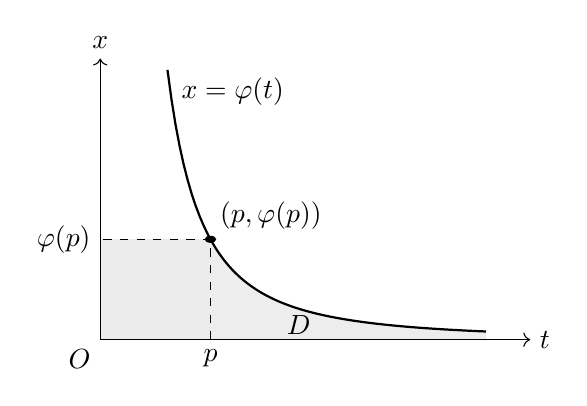
\begin{tikzpicture}[xscale=1.4,yscale=.85]
\fill[gray!15](0,0)rectangle(1,1.5);
\fill[navy!8] plot[domain=1:3.5,samples=60](\x,{1.5/(\x*\x)})--(3.5,0)--(1,0)--cycle;
\draw[->](0,0)--(3.9,0)node[right]{$t$};\draw[->](0,0)--(0,4.2)node[above]{$x$};
\draw[thick,domain=.61:3.5,samples=80]plot(\x,{1.5/(\x*\x)});
\draw[dashed](1,0)--(1,1.5)--(0,1.5);\fill(1,1.5)circle(1.5pt)node[above right]{$(p,\varphi(p))$};
\node[below]at(1,0){$p$};\node[left]at(0,1.5){$\varphi(p)$};\node[right]at(.65,3.7){$x=\varphi(t)$};\node at(1.8,.22){$D$};\node[below left]at(0,0){$O$};
\end{tikzpicture}\par{\small 图 6.5.1\quad 反函数与面积的示意（重绘，非精确函数曲线）}
\end{minipage}\end{center}
\textbf{注 6.5.3}\quad 实际上，上述证明给出归一化 $a=1$ 下更好的不等式
\begin{equation}
\int_0^\infty\varphi^2+\int_0^\infty\psi^2>\frac{8\sqrt3}{9}.\tag{6.5.7}
\end{equation}
原书称此常数仍非最佳，进一步研究的最佳常数在 $1.82649$ 与 $1.88885$ 之间。
\ednote{本注按原书历史说明保留，常数针对归一尺度 $a=1$；未独立验证上述数值，也不称其为当前最佳结果。}

\entry{例 6.5.6}{第四届全国初赛题}{pp.338—339（上半页）}
设 $f$ 在 $[0,\infty)$ 上连续可导，$f(0)>0$，$f'\ge0$。若 $\int_0^\infty\dd x/(f(x)+f'(x))$ 收敛，证明 $\int_0^\infty\dd x/f(x)$ 收敛。
\prooftext 对 $A>0$，有
\begin{align*}
0\le\int_0^A\frac1f-\int_0^A\frac1{f+f'}
&=\int_0^A\frac{f'}{f(f+f')}\le\int_0^A\frac{f'}{f^2}\\
&=\int_0^A\left(-\frac1f\right)'=\frac1{f(0)}-\frac1{f(A)}<\frac1{f(0)}.
\end{align*}
所以
\[
\int_0^A\frac1f<\int_0^\infty\frac1{f+f'}+\frac1{f(0)}.
\]
由非负函数积分的有界性判据，原积分收敛。
\ednote{原书差值前印作 $0<$；当 $f$ 初段为常值时可取零，此处按 $f'\ge0$ 规范为非严格非负号。}

\entry{例 6.5.7}{第七届全国初赛题}{pp.339—340}
设 $f$ 为 $[0,\infty)$ 上有界连续函数，$h$ 在 $[0,\infty)$ 上连续，且 $\int_0^\infty|h(t)|\dd t=a<1$。构造
\[
g_0(x)=f(x),\quad g_n(x)=f(x)+\int_0^xh(t)g_{n-1}(t)\dd t,\quad n=1,2,\ldots.
\]
证明 $\{g_n\}$ 收敛于连续函数 $g$，并求 $g$。
\prooftext 记 $M=\sup_{x\ge0}|f(x)|$，则 $|g_0|\le M$。若
$|g_{n-1}|\le(1+a+\cdots+a^{n-1})M$，则由递推式，
\begin{align*}
|g_n(x)|&\le|f(x)|+\int_0^x|h(t)||g_{n-1}(t)|\dd t\\
&\le M+\int_0^x|h(t)|(1+a+\cdots+a^{n-1})M\dd t\\
&\le M+a(1+a+\cdots+a^{n-1})M=(1+a+\cdots+a^n)M,\quad\forall x\ge0.
\end{align*}
因此 $|g_n|\le(1-a^{n+1})M/(1-a)$。再由递推式，
\[
g_n-g_{n-1}=\int_0^xh(t)[g_{n-1}(t)-g_{n-2}(t)]\dd t,
\]
故
\begin{align*}
\sup|g_n-g_{n-1}|&\le a\sup|g_{n-1}-g_{n-2}|\\
&\le a^{n-1}\sup|g_1-g_0|\le a^nM.
\end{align*}
因为 $a\in[0,1)$，函数项级数 $\sum_{n=1}^\infty(g_n-g_{n-1})$ 在 $[0,\infty)$ 上一致收敛。因此 $g_n$ 一致收敛，极限 $g$ 连续。在递推式中令 $n\to\infty$，得
\[
g(x)=f(x)+\int_0^xh(t)g(t)\dd t.
\]
解此积分方程，得到
\[
g(x)=f(x)+e^{H(x)}\int_0^xe^{-H(t)}h(t)f(t)\dd t,
\qquad H(x)=\int_0^xh(t)\dd t,\quad x\ge0.
\]

\end{document}
